% =====================================================================
%  draft.tex  —  리셀 시장 미디어 선행 지표 연구
%  작성 범위: 초록 · 서론 · 관련 연구 · 방법론 · 결과 · 논의 · 결론 · 부록
% =====================================================================
\documentclass[11pt, a4paper, twocolumn]{article}

% ----- 한글 -----
\usepackage[hangul]{kotex}
\usepackage{setspace}
\onehalfspacing

% ----- 일반 -----
\usepackage[margin=2.5cm]{geometry}
\usepackage{amsmath, amssymb}
\usepackage{booktabs}
\usepackage{graphicx}
\usepackage{hyperref}
\usepackage{natbib}
\usepackage{enumitem}
\usepackage{caption}
\usepackage{subcaption}
\usepackage{multirow}
\usepackage{dblfloatfix}        % 2-column spanning float을 페이지 하단에도 배치 가능
\usepackage[protrusion=true,expansion=false]{microtype}  % 한글 폰트 호환 위해 expansion off
\captionsetup{font=small, labelfont=bf}

% --- floats 배치 비율 조정 (두 컬럼에서 표/그림이 마지막 페이지로 몰리는 것 방지) ---
\renewcommand{\topfraction}{0.9}
\renewcommand{\bottomfraction}{0.7}
\renewcommand{\textfraction}{0.1}
\renewcommand{\floatpagefraction}{0.7}
\renewcommand{\dbltopfraction}{0.9}
\renewcommand{\dblfloatpagefraction}{0.7}
\setcounter{topnumber}{3}
\setcounter{bottomnumber}{2}
\setcounter{totalnumber}{5}
\setcounter{dbltopnumber}{3}

% ----- 메타 -----
\title{미디어 채널은 리셀 시장 가격을 선행하는가? \\
       \large 자산 유형별 Granger 인과성 분석과 머신러닝 검증}
\author{[저자명]\thanks{[소속·이메일]}}
\date{}

\begin{document}
\maketitle

% =====================================================================
\begin{abstract}
\noindent
스니커즈, 트레이딩 카드, 빌딩 블록(레고)으로 대표되는 리셀(resell) 시장은
지난 5년간 글로벌 단위로 빠르게 성장하였으나, 가격 형성에 영향을 미치는
정보 채널에 대한 실증 연구는 제한적이다. 본 연구는 다섯 가지 미디어 채널
---검색 트렌드(Google Trends), 뉴스 보도량(GDELT volume), 뉴스 감성
(GDELT tone), YouTube 조회수, YouTube 댓글 감성(FinBERT)---이 리셀
자산 가격을 \emph{선행}하는지, 그리고 \emph{선행 채널 구성이 자산
유형마다 다른지}를 검증한다.

세 자산군(스니커즈·카드·레고)에서 각 5개 아이템, 총 15개 아이템에 대해
2022년 1월부터 2025년 12월까지 48개월 월별 패널을 구축하였다. 자산별로
다섯 채널 각각에 대해 단독(bivariate) Granger 인과성 검정을 수행하여
3자산 $\times$ 5채널 $=$ 15회의 유의성을 평가하였다. 자산별 유의 채널
집합 간 Jaccard 유사도를 통해 채널 구성의 이질성을 정량화하였으며,
연속된 후속 단계로 XGBoost와 Diebold--Mariano 검정을 활용하여 선별
채널 모형의 예측 성능을 평가한다.

실증 분석 결과, 15회 Granger 검정 중 4회가 유의($p<0.05$), 1회가 경계
수준($0.05\leq p<0.10$)으로 관찰되었다. 스니커즈에서는 Google Trends(CH1),
뉴스 감성(CH3), YouTube 조회수(CH4)가, 카드에서는 Google Trends(CH1)가
가격을 선행하는 \emph{잠정적} 증거가 확인되었다(RQ1). 자산쌍 간 Jaccard
유사도는 sneakers--cards $=0.333$, 그 외 $=0.000$으로, 자산 유형 간
유의 채널 구성이 대체로 상이하되 검색 트렌드(CH1)에서 부분적 중복이
존재한다(RQ2). 자산-평균 검정과 RQ3 머신러닝 단계의 분석 단위 불일치를
보완하기 위해 5개 아이템을 횡단면으로 두는 \citet{dumitrescuhurlin2012}
패널 Granger 검정을 보충 수행하였으며, BH 보정 후에도 자산-평균과 DH
양쪽에서 일관되게 유의한 채널은 cards--CH1 한 조합으로 집약된다. 보충적으로 BH 보정 후 유의가 유지된 두 조합에 대한 직교화
충격반응함수는 \emph{1\textasciitilde2개월 선행 + 4개월 내 감쇄}의
공통 패턴을 보이되 부호가 정반대로 나타나, cards--CH1은 양(+10.80,
1개월), sneakers--CH3는 음(-2.82, 1개월)의 가격 반응이 95\% 잔차 부트스트랩
신뢰구간에서 0을 포함하지 않았다. XGBoost 예측 비교에서는 15개 아이템 중 11개(73\%)에서
Granger 선별 모형(Model B)과 전채널 모형(Model A) 간 \emph{DM 검정상}
통계적으로 유의한 차이가 없었으나, 자산별 평균 RMSE는 sneakers·lego에서
Model A가 일관되게 낮고 2개 아이템(\textsf{jordan1}, \textsf{falcon})에서는
Model A가 유의하게 우수하여, Granger 선별은 ``우수''보다 ``큰 손해 없이
간결화 가능''에 가까운 절제된 해석을 지지한다(RQ3). SHAP 분석에서는 채널 변수의 절대
기여도가 가격 모멘텀 변수보다 현저히 작았으며, Granger 순위와 SHAP 순위
간 불일치가 관찰되었다. 이는 선형 인과성 검정과 비선형 예측 모형의 측정
대상 차이에서 기인하며 \S\ref{sec:discussion-shapgranger}에서 다룬다.
표본 크기($N=48$)와 다중 검정 구조를 고려할 때, 본 연구의 결과는
\emph{탐색적} 발견으로 해석되어야 한다.

\medskip\noindent
\textbf{핵심어:} 리셀 시장, Granger 인과성, 미디어 선행 지표,
GDELT, Google Trends, FinBERT, XGBoost, SHAP
\end{abstract}

\begin{abstract}[english]
\noindent
The resell market for sneakers, trading cards, and LEGO sets has grown
rapidly on a global scale over the past five years, yet empirical research
on the information channels that shape price formation remains limited.
This study examines whether five media channels---Google Trends search
interest, GDELT news volume, GDELT news sentiment, YouTube view counts,
and YouTube comment sentiment (FinBERT)---\emph{lead} resell asset prices,
and whether the composition of significant leading channels differs across
asset types.

We construct a 48-month monthly panel from January 2022 to December 2025
covering 15 items (5 per asset class: sneakers, trading cards, and LEGO
sets). Bivariate Granger causality tests are conducted for each
asset-type $\times$ channel pair (3 assets $\times$ 5 channels $=$ 15 tests).
Jaccard similarity between asset-specific sets of significant channels
quantifies compositional heterogeneity (RQ2), and XGBoost with
Diebold--Mariano tests evaluates the predictive performance of
Granger-selected channel models versus full-channel models (RQ3).

Out of 15 Granger tests, 4 are significant ($p<0.05$) and 1 is marginal
($0.05\leq p<0.10$). Tentative evidence of price leadership is found for
Google Trends, news sentiment, and YouTube views in sneakers, and for
Google Trends in trading cards (RQ1). Jaccard similarity is 0.333 for
the sneakers--cards pair and 0.000 otherwise, indicating largely
heterogeneous channel compositions across asset types (RQ2). To
reconcile the analytical-unit gap between asset-level Granger tests and
the item-level XGBoost stage, we additionally apply the panel Granger
non-causality test of \citet{dumitrescuhurlin2012} treating the five
items within each asset as cross-sections; after BH correction, only
\emph{cards--CH1} remains significant in both the asset-mean Granger and
the panel DH test, while the strongest asset-mean finding
(sneakers--CH3) is reduced to non-significance under DH, suggesting
possible aggregation-induced amplification. A complementary
six-variable VAR with block and individual Granger tests (controlling
for cross-channel multicollinearity) confirms that the only finding
surviving BH correction across all three tests is \emph{cards--CH1},
which we report as the most robust asset-common leading channel.
Supplementary orthogonalised impulse-response functions for the two
BH-robust channels show a common short-lead pattern (peak at 1--2 months,
decay within 4 months) but opposite signs: cards--CH1 produces a positive
price response ($+10.80$ at horizon 1) while sneakers--CH3 produces a
negative one ($-2.82$ at horizon 1), with 95\% residual-bootstrap CIs
excluding zero in both cases. In XGBoost
comparisons, 11 of 15 items (73\%) show no statistically significant
difference between Granger-selected (Model B) and full-channel (Model A)
models by DM test; however, asset-level mean RMSE consistently favors
Model A for sneakers and LEGO, supporting a tempered interpretation that
Granger selection reduces channel count without major predictive loss
rather than achieving superiority (RQ3). Given the sample size ($N=48$)
and multiple testing structure, all findings should be regarded as
\emph{exploratory}.

\medskip\noindent
\textbf{Keywords:} Resell market, Granger causality, Media leading
indicators, GDELT, Google Trends, FinBERT, XGBoost, SHAP
\end{abstract}

% =====================================================================
\section{서론}\label{sec:intro}

스니커즈 리셀 플랫폼 \textit{StockX}, 트레이딩 카드 그레이딩 시장
(PSA 10), 그리고 단종(retired) 레고 세트 등은 한정된 공급, 표준화된
품질 보증, 그리고 디지털 거래 인프라의 결합을 통해 \emph{대안 자산
(alternative asset)}의 한 축으로 자리잡았다. 거래량과 가격 변동성은
주식·암호화폐 시장에 비해 작지만, 가격 결정 구조 자체는 정보 비대칭과
\emph{관심(attention)}---즉 잠재 구매자·수집가의 인지 노출량---에
민감하다는 점에서 금융 시장과 본질을 공유한다.

기존 금융 연구는 검색 트렌드와 거래량의 관계\citep{daengelberggao2011,
preismoatstanley2013}, 뉴스 텍스트의 감성과 수익률의 관계
\citep{tetlock2007, loughranmcdonald2011}, 그리고 소셜 미디어 무드와
주가 변동의 관계\citep{bollenmaozeng2011}를 충분히 축적해 왔다.
그러나 이러한 통찰이 \emph{리셀 시장}에서도 그대로 작동하는지, 그리고
자산 유형(스니커즈·카드·레고)에 따라 \emph{어떤 채널}이 선행적
역할을 하는지는 거의 연구되지 않았다.

본 연구는 다음 세 가지 연구 문제와 대응 가설을 제기한다.

\begin{description}[leftmargin=1.6em, labelindent=0.4em]
  \item[\textbf{RQ1}] 다섯 가지 미디어 채널은 각 리셀 자산의 가격을
        Granger 의미에서 선행하는가?
  \item[\textbf{H1}] 다섯 채널 중 적어도 일부는 리셀 자산 가격에 대해
        Granger 인과성을 보인다. 즉 단독 Granger 검정에서 귀무가설
        $H_0\colon\gamma_1=\cdots=\gamma_L=0$이 기각되는 (자산, 채널)
        조합이 존재한다.
  \item[\textbf{RQ2}] 유의한 채널 구성이 자산 유형(스니커즈·카드·
        레고)마다 다른가?
  \item[\textbf{H2}] H1에서 유의로 판정된 채널 집합은 자산 유형 간에
        차별화된다. 자산쌍 간 Jaccard 유사도 $J<0.6$이 관찰된다.
  \item[\textbf{RQ3}] Granger 검정으로 선별된 채널만으로 학습한 예측
        모형(Model B)은 전 채널을 사용한 모형(Model A)과 동등 또는
        더 우수한 성능을 달성하는가?
  \item[\textbf{H3}] H1의 유의 채널만으로 구성한 Model B의 예측 오차는
        Model A 대비 통계적으로 구분되지 않거나 더 작다.
        Diebold--Mariano 검정에서 $p>0.10$(등가) 또는 $p<0.05$이고
        Model B에 유리한 부호가 관찰된다.
\end{description}

본 연구의 기여는 세 가지로 요약된다. 첫째, 자산 유형 단위에서 다섯
미디어 채널의 선행성을 단독 Granger 검정으로 비교하는 \emph{비교
가능한 설계}를 제시한다. 둘째, 가격 시계열 외 \emph{모든 비가격 지표는
사전에 점수 변환을 거쳐 동일 단위로 투입}함으로써, 이질적 데이터
소스 간 직접 비교의 위험을 줄였다. 셋째, 통계적 인과성 검정과 XGBoost
+ SHAP 예측 검증을 결합하여, \emph{선행성(causality lead)과 예측력
(predictive utility)을 분리}하여 평가한다.

% =====================================================================
\section{관련 연구}\label{sec:related}

\subsection{검색 관심과 자산 가격}
검색 엔진 사용량은 잠재 투자자·소비자의 \emph{능동적 정보 수요
(active information demand)}를 직접적으로 측정하는 지표로 자리잡았다.
\citet{daengelberggao2011}은 미국 종목별 Google 검색 빈도(SVI)가 산업·
시장 수준 이상의 \emph{개별 종목 관심}을 측정하며, 개인 투자자의
관심 증가는 단기 가격 압력과 장기 가격 반전 패턴 모두와 체계적으로
연관됨을 보였다. \citet{preismoatstanley2013}는 \emph{거래
행태와 검색량 간의 동적 관계}를 정량화하여, 특정 키워드(예: ``debt'')
검색의 급증이 향후 시장 하락을 선행하는 신호로 해석될 수 있음을
실증하였다. \citet{josephwintokizhang2011}은 S\&P 500 종목에 대해
검색 빈도가 \emph{비정상 수익률과 거래량 모두}를 예측한다는 결과를
보고하였고, \citet{vlastakismarkellos2012}는 검색량으로 근사한 정보
수요가 변동성·거래량과 양의 관계를 가짐을, \citet{vozlyublennaia2014}는
검색 기반 관심의 단기 충격이 지수 수익률 패턴을 변화시킴을 보고
하였다. 위키피디아·뉴스 검색 등 \emph{인접 디지털 흔적} 자료를 활용한
연구도 누적되었는데, \citet{bordinoetal2012}는 Yahoo Finance 종목
페이지에 대한 검색 쿼리가 거래량을 예측함을 보였으며, \citet{moatetal2013}와
\citet{curmeetal2014}는 위키피디아 페이지 조회 패턴이 주식 시장의 가격
변동을 선행하는 행동학적 신호를 담고 있음을 보고하였다.

이들 연구는 일관되게 \emph{검색·조회는 잠재 수요의 선행 지표}라는
직관을 지지하며, 본 연구는 동일 직관을 \emph{리셀 시장 아이템 단위}로
이식한다. 다만 주식 시장 연구가 종목 단위 일별·주별 검정에 주로
집중한 반면, 본 연구는 자산 \emph{유형 수준}의 월별 검정으로 단위를
변경함으로써, 검색이 \emph{어떤 자산군에서 가장 강한 선행 신호}로
작동하는지를 비교 가능하도록 설계한다.

\subsection{뉴스 텍스트와 감성 분석}
뉴스의 텍스트적 정보 내용이 자산 가격에 미치는 영향에 관한 실증은
\citet{tetlock2007}로부터 본격화되었다. 그는 \textit{Wall Street
Journal}의 ``Abreast of the Market'' 칼럼에서 추출한 비관 척도가
다우존스 지수의 단기 수익률을 선행적으로 예측한다는 결과를 보고하였고,
\citet{tetlocksaarmacskassy2008}은 기업 관련 뉴스의 부정적 단어 빈도가
회계적 펀더멘털(이익, 거래량)에 대한 \emph{추가 정보}를 담고 있음을
보였다. \citet{garcia2013}는 1905--2005년 \textit{New York Times}의
경제 칼럼 감성을 분석하여, \emph{경기 침체기일수록} 미디어 감성의
수익률 예측력이 강화된다는 \emph{상태 의존성}을 발견하였다.
\citet{engelbergparsons2011}은 동일 사건에 대한 지역별 보도량 차이를
\emph{외생적 식별 전략}으로 활용하여, 미디어 보도 자체가 거래 행태에
\emph{인과적} 영향을 미친다는 강한 증거를 제시하였다.

방법론 측면에서 \citet{loughranmcdonald2011}은 일반 사전(Harvard
General Inquirer)이 금융 텍스트에 부적합하다는 점을 지적하며 금융
도메인 사전을 제안하였고, \citet{kearneyliu2014}와
\citet{loughranmcdonald2016}은 금융 텍스트 감성 분석의 방법론적
조류를 종합적으로 정리하였다. 한편 \citet{hestonsinha2017}은 뉴스 보도량
대비 \emph{감성의 부호}가 수익률 예측에 미치는 한계 기여를 정량화하여,
``보도되었다''와 ``어떻게 보도되었다''를 분리 평가하는 설계의 중요성을
강조하였다.

본 연구의 CH2(뉴스 보도량)와 CH3(뉴스 감성)는 위 두 차원---\emph{보도의
양과 어조}---을 GDELT 프로젝트\citep{leetaharvardgdelt}의
\texttt{timelinevolnorm}과 \texttt{timelinetone}으로 각각 측정한다.
GDELT 톤은 도메인 특화 사전이 아닌 일반 감성 점수라는 한계를
지니나, 본 연구의 분석 기간(2022--2025) 동안 4년 단위의 역사 자료를
무료로 일관되게 제공한다는 운용상 장점이 크다(자세한 한계 논의는
\S\ref{sec:method-channels} 및 \S\ref{sec:discussion-limit} 참조).

\subsection{소셜 미디어·이용자 생성 콘텐츠와 자산 가격}
이용자 생성 콘텐츠(user-generated content)는 미디어 콘텐츠의 양과
질 모두를 \emph{대중의 시각에서} 측정한다는 점에서 전통 뉴스와
구별된다. \citet{antweilerfrank2004}는 Yahoo Finance 주식 게시판
메시지의 정보 내용이 변동성과 거래량을 예측함을 보였으나, 평균
수익률에 대한 효과는 약함을 보고하였다. \citet{bollenmaozeng2011}은
트위터 무드 지표가 다우존스 지수의 단기 변동을 예측함을 보였으며,
\citet{sprengeretal2014}는 종목별 트위터 메시지의 감성·메시지 수
모두 비정상 수익률과 거래량을 예측함을 정량적으로 입증하였다.
이들 연구는 공통적으로 \emph{이용자 콘텐츠의 양과 질이 시장 관심을
반영한다}는 직관을 지지한다.

본 연구의 CH4(YouTube 조회수)와 CH5(YouTube 댓글 감성)는 동일 직관을
\emph{영상 플랫폼}으로 확장한다. CH4는 자산-아이템별 ``resell,
review'' 키워드를 기반으로 수집한 영상의 월별 조회수 합산(아이템 내
z-score)으로, \emph{정보 탐색 의도}를 측정한다. CH5는 조회수 상위
영상의 영어 댓글에 대해 \citet{araci2019finbert}의 FinBERT를 적용하여
$P(\text{pos})-P(\text{neg})$의 월 평균으로 산출한다. FinBERT는
\citet{devlinetal2019}의 BERT를 금융 도메인 텍스트로 추가 학습한
모형으로, 일반 도메인 감성 분류기 대비 금융 어휘에 대한 분류 정확도가
높다는 점에서 채택하였다.

\subsection{머신러닝 기반 예측과 해석}
표 형식 시계열의 분류·회귀 과제에서 트리 부스팅 모형은 강건한
성능을 보여 왔으며, 그중 XGBoost\citep{chenguestrin2016}는 효율적
구현과 정규화 항을 결합하여 사실상 표준 도구로 자리잡았다. 금융
영역에서도 \citet{gukellyxiu2020}은 미국 주식 횡단면 수익률 예측에
다양한 머신러닝 모형(선형, 트리, 신경망)을 비교 적용하여, 트리
계열과 얕은 신경망이 일관되게 선형 회귀 대비 우월한 예측력을
보임을 보고하였다.

머신러닝 모형의 해석 가능성에 관해서는, SHAP\citep{lundberglee2017}이
게임 이론의 Shapley 값을 모형 예측에 적용하여 \emph{개별 예측에
대한 변수별 한계 기여도}를 통일적으로 분해하는 표준 도구로 자리잡았다.
SHAP은 트리 부스팅과 결합 시 정확한 계산이 가능하며, 본 연구는
이를 통해 채널별 평균 $|\text{SHAP}|$를 ``전역(global) 변수 중요도''로
사용한다. 본 연구는 \emph{Granger 검정에 의한 통계적 선행성}과
\emph{XGBoost+SHAP에 의한 예측 기여도}를 같은 데이터로 직접 대조함
으로써, 인과성과 예측력을 분리하여 평가하는 설계상의 차별점을
가진다.

\subsection{대안 자산·리셀 시장 연구의 공백}
대안 자산 수익률 연구는 다양한 수집품 클래스를 누적해 왔다.
\citet{burtonjacobsen1999}은 수집품 투자 수익률 측정 방법론을 정리하여
수집품이 양의 실질 수익률을 보이나 주식 대비 위험이 크다는 점을
보였고, \citet{meimoses2002}는 반복 거래 자료로 1875--2000년 미술
가격 지수를 추정해 미술이 채권을 상회하나 주식보다는 낮은 수익률을
가짐을 보고하였다. \citet{renneboogspaenjers2013}은 1957--2007년
헤도닉 회귀로 미술 시장의 실질 연 수익률을 약 4\%로 추정하면서
소비자 신뢰와 미술 시장 정서가 가격을 예측함을 보였다.
\citet{dimsonrousseauspaenjers2015}은 보르도 와인의 실질 연 수익률이
4.1\%로 채권·미술·우표를 상회함을 보였다.

본 연구가 다루는 세 자산군에 대해서는,
\citet{dobrynskayakishilova2022}이 1987--2015년 eBay 거래 자료를 바탕으로
LEGO 세트의 연 평균 명목 수익률을 약 11\%(실질 8\%)로 추정하여 LEGO가
주식·채권·금·일부 대안 자산을 상회한다는 결과를 보고하였다. 스니커즈
재판매 시장에 대해서는 \citet{radityaetal2021}이 StockX 데이터에
선형 회귀와 랜덤 포레스트를 적용해 재판매 가격을 예측하는 등 기계
학습 기반 가격 예측 연구가 진행 중이며, 트레이딩 카드(포켓몬·스포츠
카드 등)에 대한 연구는 학위논문 수준의 사례 분석이 산발적으로 존재한다.

이들 선행 연구는 개별 자산 \emph{수익률}을 측정하는 데 집중한 반면,
\emph{여러 자산군을 동일 기간·동일 채널 정의로 직접 비교하여 미디어
채널의 선행성을 평가}한 실증 연구는 저자들이 확인한 범위에서 매우
제한적이다. 본 연구는 이 공백을 메우는 것을 1차 목표로 한다.

% =====================================================================
\section{방법론}\label{sec:method}

\subsection{전체 설계}\label{sec:method-design}

본 연구는 다음 단계로 구성된다.

\begin{enumerate}[leftmargin=1.6em]
  \item 가격·채널 데이터 수집(STEP 01--04).
  \item 채널별 점수 변환 및 결측 처리(STEP 05--06).
  \item ADF 정상성 검정 및 필요 시 1차 차분(STEP 07).
  \item 자산별 단독 Granger 인과성 검정(STEP 08).
  \item Jaccard 유사도를 통한 자산별 유의 채널 구성 비교(STEP 08).
  \item XGBoost + SHAP + Diebold--Mariano 검정을 통한 예측 검증(STEP 09).
\end{enumerate}

\subsection{데이터}\label{sec:method-data}

\textbf{기간 및 단위.} 분석 기간은 2022년 1월부터 2025년 12월까지의
48개월이며, 모든 변수는 월(month) 단위로 집계된다. 자산군은 스니커즈
(\textsf{sneakers}), 트레이딩 카드(\textsf{cards}), 레고(\textsf{lego})
의 셋이며, 각 자산군에 대해 5개 대표 아이템을 선정하여 총 15개 아이템
$\times$ 48개월 $=$ 720개 아이템-월 패널을 구축하였다.

\textbf{아이템 선정 기준.} (i) 2022년 이전부터 시장이 형성되어 48개월
연속 가격 관측이 가능할 것, (ii) 자산군 내에서 거래 빈도와 인지도가
충분히 높을 것, (iii) Google Trends에서 검색량이 측정 가능할 것
(0이 다수 발생하는 후보는 제외)을 동시에 만족시키는 아이템을 자산군별
5개씩 선정하였다(표 \ref{tab:items}).

\begin{table*}[!tbp]
\centering\small
\caption[선정된 15개 아이템과 출처]{\textbf{선정된 15개 아이템과
출처.} 본 연구의 분석 대상은 스니커즈·트레이딩 카드·레고의 세 자산군이며,
각 자산군에서 (i) 2022년 이전부터 시장이 형성되어 48개월 연속 가격
관측이 가능하고, (ii) 자산군 내 거래 빈도와 인지도가 충분히 높으며,
(iii) Google Trends에서 검색량이 측정 가능한 5개 대표 아이템을 선정
하였다. 가격 출처는 자산군별로 다르며, 스니커즈는 \emph{StockX}의
미국 사이즈 10 거래가, 카드는 \emph{PriceCharting}의 PSA 10 등급
가격, 레고는 \emph{BrickRanker}의 신품 봉인(new sealed) 가격을
사용하였다. \textsf{sneakers\_jordan1}과 \textsf{cards\_charizard1}은
초기 후보 아이템의 출시일·URL 문제로 교체되었으며, 자세한 변경
이력은 부록 표~\ref{tab:item-history}에 정리하였다.}
\label{tab:items}
\begin{tabular}{llll}
\toprule
자산군 & ID & 아이템 & 출처 \\
\midrule
sneakers & sneakers\_jordan1 & Air Jordan 1 Retro High OG Bordeaux & StockX \\
sneakers & sneakers\_panda   & Nike Dunk Low Panda                  & StockX \\
sneakers & sneakers\_yeezy   & Yeezy 350 V2 Zebra                   & StockX \\
sneakers & sneakers\_travis  & Travis Scott Jordan 1                & StockX \\
sneakers & sneakers\_nb550   & New Balance 550 White/Green          & StockX \\
\midrule
cards    & cards\_charizard1 & Charizard VMAX, Shining Fates SV107  & PriceCharting (PSA 10) \\
cards    & cards\_charizard2 & Charizard GX, Hidden Fates           & PriceCharting (PSA 10) \\
cards    & cards\_umbreon    & Umbreon VMAX Alt Art                 & PriceCharting (PSA 10) \\
cards    & cards\_rayquaza   & Rayquaza VMAX Alt Art                & PriceCharting (PSA 10) \\
cards    & cards\_pikachu    & Pikachu VMAX                         & PriceCharting (PSA 10) \\
\midrule
lego     & lego\_falcon      & Millennium Falcon 75192              & BrickRanker (new sealed) \\
lego     & lego\_hogwarts    & Hogwarts Castle 71043                & BrickRanker (new sealed) \\
lego     & lego\_titanic     & Titanic 10294                        & BrickRanker (new sealed) \\
lego     & lego\_porsche     & Porsche 911 42096                    & BrickRanker (new sealed) \\
lego     & lego\_bugatti     & Bugatti Chiron 42083                 & BrickRanker (new sealed) \\
\bottomrule
\end{tabular}
\end{table*}

\textbf{가격 자료.} 스니커즈는 StockX의 미국 사이즈 10 거래가, 카드는
PriceCharting의 PSA 10 등급 가격, 레고는 BrickRanker의 신품 봉인
가격을 사용하였다. 월별 평균 가격(\textsf{mean\_price})과 거래 건수
(\textsf{tx\_count})를 추출하였으며, 거래 건수가 3 미만인 월은 선형
보간으로 대체하였다.\footnote{연속 3개월 이상 \textsf{tx\_count}가 3
미만인 경우는 해당 기간을 제외 검토하였다. 본 연구의 15개 아이템 중
이 기준에 해당된 사례는 \textsf{sneakers\_yeezy}(StockX 거래량 표본
추출 아티팩트로 인한 4개월 결측, 선형 보간으로 처리)이며 한계 절에
명시한다.}

\textbf{한계 및 자료 변경 내역.} 본 패널은 다음의 자료원·아이템 변경을
거쳐 확정되었다. (i) 레고는 PriceCharting이 2023년 11월 이후 데이터만
보유하여 BrickRanker로 전환. (ii) 일부 레고 아이템은 Google Trends 0
빈도가 과다하여 대체(자세한 변경 이력은 부록 표~\ref{tab:item-history} 참조).
(iii) \textsf{sneakers\_jordan1}은 \emph{Chicago Lost \& Found}(2022-11
출시)이 초기 7개월 가격이 부재하여 \emph{Bordeaux}로 변경.
(iv) \textsf{cards\_charizard1}은 \emph{Evolving Skies \#74}의 URL이
다른 카드로 리다이렉트되어 \emph{Shining Fates SV107}로 변경.

\subsection{채널 정의 및 점수 변환}\label{sec:method-channels}

다섯 채널의 정의와 변환 규칙은 표 \ref{tab:channels}와 같다.
\textbf{원시 데이터를 Granger 검정에 직접 투입하지 않으며}, 모든 채널은
사전에 다음의 표준 변환을 거쳐 동일 단위로 비교 가능하도록 정렬한다.

\begin{table*}[!tbp]
\centering\small
\caption[채널 정의 및 점수 변환]{\textbf{다섯 미디어 채널의 정의,
자료원, 점수 변환 규칙, 그리고 최종 범위.} 본 연구는 원시 자료를
Granger 검정에 직접 투입하지 않으며, 모든 채널은 사전에 표준 변환을
거쳐 동일 단위로 비교 가능하도록 정렬된다. CH1(Google Trends)은
\texttt{pytrends} API로 영문 키워드의 월별 검색 관심도를 수집한 뒤
월평균을 취한다. CH2(뉴스 보도량)와 CH3(뉴스 감성)는 GDELT 프로젝트의
\texttt{timelinevolnorm}과 \texttt{timelinetone} 모드에서 일별 자료를
받아 월평균으로 집계하며, CH3는 원범위($-10\sim+10$)를 10으로 나누어
$-1\sim+1$로 재정규화한다. CH4(YouTube 조회수)는 \texttt{publishedAt}이
해당 월에 속하는 영상의 조회수 합산을 \texttt{log1p} 변환한 뒤 아이템
내 z-score를 취한다(누적 왜곡 방지). CH5(YouTube 댓글 감성)는 조회수
상위 영상의 영어 댓글에 대해 FinBERT로 $P(\text{pos})-P(\text{neg})$를
계산한 뒤 월 평균을 취한다. CH3의 GDELT 대체 사유와 한계는
\S\ref{sec:method-channels}에서 상세 논의한다.}
\label{tab:channels}
\begin{tabular}{l l l p{4.5cm} l}
\toprule
ID & 이름 & 자료원 & 변환 방식 & 범위 \\
\midrule
CH1 & Google Trends     & pytrends                       & 월평균                                                         & 0--100 \\
CH2 & 뉴스 보도량        & GDELT \texttt{timelinevolnorm} & 일별 $\rightarrow$ 월평균                                      & 0--1 \\
CH3 & 뉴스 감성          & GDELT \texttt{timelinetone}    & 월평균 $\div 10$                                               & $-1\sim+1$ \\
CH4 & YouTube 조회수     & YouTube Data API               & 월별 조회수 합산 $\rightarrow$ \texttt{log1p} $\rightarrow$ 아이템 내 z-score & z-score \\
CH5 & YouTube 댓글 감성  & YouTube + FinBERT              & $P(\text{pos}) - P(\text{neg})$ 월평균                         & $-1\sim+1$ \\
\bottomrule
\end{tabular}
\end{table*}

\textbf{CH1 (Google Trends).} \texttt{pytrends}를 사용하여 아이템별
영문 키워드(예: ``\textit{Jordan 1 Bordeaux}'')의 월별 평균 검색
관심도를 수집하였다. 지역은 전 세계(\texttt{geo=''})로 설정하였다.

\textbf{CH2·CH3 (GDELT).} CH2는 \texttt{timelinevolnorm} 모드를
사용하여 일별 정규화된 보도량을 받고 월평균을 취하며, CH3는
\texttt{timelinetone} 모드의 일별 평균 톤(원범위 $-10\sim+10$)을 월평균
취한 뒤 10으로 나누어 $-1\sim+1$로 재정규화한다.

\textbf{CH3 한계.} 원래 설계는 NewsAPI로 수집한 도메인 텍스트에
FinBERT를 적용하는 것이었으나, NewsAPI 무료 플랜의 30일 역사 자료
제한으로 4년 길이 수집이 불가능하여 GDELT \texttt{timelinetone}으로
대체하였다. GDELT 톤은 일반 어휘 기반 자동 산출 점수로, 도메인 특화
감성 분석 대비 신호 대 잡음비가 낮을 가능성이 있다(한계 절 명시).

\textbf{CH4 (YouTube 조회수).} \texttt{search.list}와
\texttt{videos.list} 두 엔드포인트를 결합하여 검색을 수행한다. 누적
왜곡을 방지하기 위해 영상의 \texttt{publishedAt}이 \emph{해당 월
1일부터 말일 사이}인 영상만을 집계하며, 이를 위해
\texttt{publishedAfter}와 \texttt{publishedBefore} 파라미터로 구간을
강제한다. 검색 키워드는 자산-아이템별로 \emph{resell, review, price}
등 정보 탐색형 어휘를 결합하여 사전에 고정하였다(예: ``\textit{Jordan
1 Bordeaux resell review}'', ``\textit{LEGO Millennium Falcon 75192
review sealed price}''; 전체 목록은 \texttt{scripts/collect\_youtube.py}
참조). 월별 영상 조회수 합산을
\texttt{log1p}로 변환한 뒤 아이템 내 z-score를 취하여 \textsf{score\_ch4}로
정의한다.\footnote{\textit{스케일 일관성 주.} 본 변환으로 산출된
\textsf{score\_ch4}는 Granger 검정용 자산 시계열(아이템 평균)에 그대로
사용된다. XGBoost 단계(\S\ref{sec:method-ml})에서는 \emph{모든 채널
점수}가 추가로 전역 z-score 정규화를 거치므로, CH4는 이중 정규화
(아이템 내 $\to$ 전역)된다. 이는 채널 간 스케일 통일을 위한 의도된
처리이며 모형의 단조 변환 불변성으로 인해 트리 기반 XGBoost 예측에는
실질적 영향이 없으나, SHAP 절대값 해석 시 본 처리를 감안해야 한다.}

\textbf{CH4 의미 한계.} 검색 키워드가 \emph{resell·review} 중심이므로,
CH4는 일반 팬덤·hype보다는 \emph{정보 탐색 의도(information-seeking
intent)}를 측정한다. 이 점은 결과 해석에서 명시한다.

\textbf{CH5 (YouTube 댓글 감성).} 조회수 상위 15개 영상 각각에서
관련도(\texttt{order=relevance}) 기준 30개씩 댓글을 수집한 뒤,
\texttt{langdetect}로 영어 댓글만 필터링한다. 필터링된 댓글에 대해
\texttt{ProsusAI/finbert}\citep{araci2019finbert}로 $P(\text{pos})$,
$P(\text{neg})$, $P(\text{neu})$를 산출하고, 월 단위로
$P(\text{pos})-P(\text{neg})$의 평균을 \textsf{score\_ch5}로 정의한다.

\textbf{결측 처리.} 단일 또는 2개월 연속 결측은 선형 보간으로 채우며,
3개월 이상 연속 결측은 보간하지 않고 결과 해석 시 한계로 명시한다.
GDELT 일부 아이템에서 발생한 결측은 검색 쿼리를 수정하여 재수집하였다
(부록 변경 이력 참조).

\subsection{ADF 정상성 검정}\label{sec:method-adf}

Granger 인과 검정은 시계열의 정상성을 전제로 하므로, 본 연구는 가격
및 다섯 채널 점수 각각에 대해 단위근의 부재를 사전 점검한다. 점검
도구는 \citet{dickeyfuller1979}의 Augmented Dickey--Fuller 검정이며,
귀무가설 ``단위근 존재''가 유의수준 $5\%$에서 기각되지 않는 시계열은
1차 차분된 형태로 변환한 뒤 동일 검정을 재실행한다. 자산-채널 단위로
이 절차를 반복하여 정상성 처리 결과를
\texttt{results/stationarity.csv}에 기록하고, 후속 Granger 검정에서는
차분이 필요한 시계열에 한해 일관되게 차분값을 사용한다.

\subsection{Granger 인과성 검정}\label{sec:method-granger}

\textbf{분석 단위.} 자산(asset) 수준의 \emph{대표 시계열}을 사용한다.
즉, 각 자산군에서 5개 아이템의 월별 가격과 채널 점수를 평균하여
자산-월 단위 시계열을 만들고, 이 시계열에 대해 Granger 검정을 수행한다.
이는 아이템 간 독립 검정에서 발생하는 사례별 잡음을 평균을 통해
감쇄하기 위함이며, 자산 단위 비교(RQ2)와 직접 정렬된다.

\textbf{검정 형태.} 각 (자산, 채널) 쌍을 대상으로
\citet{granger1969}의 이변량 인과 검정 절차를 적용한다. 구체적으로
가격의 자기회귀만을 포함한 제한 모형과, 여기에 한 채널의 시차값을
추가한 비제한 모형을 각각 추정한 뒤 잔차제곱합 기반 F 통계량으로
두 모형을 비교한다.
\begin{align}
  \text{(제한)}\quad   p_t &= \alpha_0 + \sum_{k=1}^{L} \alpha_k\, p_{t-k} + \varepsilon_t, \\
  \text{(비제한)}\quad p_t &= \beta_0 + \sum_{k=1}^{L} \beta_k\, p_{t-k}
                                          + \sum_{k=1}^{L} \gamma_k\, c_{t-k} + \eta_t,
\end{align}
여기서 $p_t$는 가격(필요 시 1차 차분), $c_t$는 한 미디어 채널의 점수
(필요 시 1차 차분), $L$은 래그 길이이다. 채널 간 상호작용을 RQ1
단계에서 통제하지 않기 위해 본 절에서는 채널을 한 번에 하나씩만 투입한다
(다채널 동시 투입은 \S\ref{sec:results-var}의 VAR 절에서 별도로 다룬다).
채널 시차계수 전체가 0이라는 귀무가설 $H_0:\gamma_1=\cdots=\gamma_L=0$이
기각될 때, 해당 채널이 가격을 Granger 의미에서 선행한다고 판정한다.

\textbf{래그 선택.} 후보 래그를 $\{1,2,3,4\}$로 두고 두 시계열의
이변량 VAR을 적합한 뒤, \citet{schwarz1978} 기준(BIC)이 최소화되는
래그를 자산-채널 조합별로 채택한다. 그래도 유의 결과가 전혀 관찰되지
않는 조합에 한해 보조 진단으로 $L=5,6$까지 확장하여 검정을 반복한다.

\textbf{판정 기준.} 본 연구는 유의성 판정을 raw $p$-값 하나로 단순화
한다. $p<0.05$는 SIGNIFICANT, $0.05\leq p<0.10$은 MARGINAL(탐색적
참고), $p\geq 0.10$은 NOT\_SIG로 표기한다. $F$ 값 자체는 효과 크기를
가늠하기 위한 부수 지표로만 함께 보고하며, ``$F \geq 4.0$'' 같은 비표준
임계값은 컷오프 자의성을 회피하기 위해 사용하지 않는다.

\noindent\textit{다중비교 보정에 관한 주.}\footnote{본 단계에서
이루어지는 15회 검정에 \citet{benjaminihochberg1995}의 FDR 보정을
적용하면 일부 유의 판정이 약화될 수 있다. 그럼에도 raw $p$-값을 1차
판정 도구로 채택한 근거는 세 가지이다. 첫째, Granger 인과성을 활용한
응용 계량 문헌에서 단독 검정의 raw $p$-값 보고는 표준 관행에 속한다.
둘째, 본 연구의 검정 단위는 \emph{서로 다른 자산-채널 조합}으로
구성되며, 동일 가설을 반복 표본으로 평가하는 구조가 아니다. 셋째, 본
단계의 일차 목적이 후속 머신러닝에 투입할 채널의 \emph{선별}이며,
지나치게 보수적인 FDR 적용은 잠재적으로 유용한 신호까지 과대 배제할
위험이 있다. 그럼에도 결과의 강건성 점검을 위해 BH 보정 결과를
부록 표로 함께 제시한다.}

\subsection{패널 Granger 인과성 검정 (Dumitrescu--Hurlin)}\label{sec:method-dh}

자산-평균 시계열을 사용하는 \S\ref{sec:method-granger}의 설계는 분석을
단순화하지만 두 가지 잠재적 약점을 갖는다. 첫째, 자산 내 아이템 5개의
시계열을 산술 평균함으로써 \emph{아이템 간 신호의 이질성}을 측정 단계에서
이미 제거한다. 둘째, RQ3의 XGBoost는 아이템 단위(15개 패널)로 학습되므로,
Granger(자산 단위)와 \emph{분석 단위가 일치하지 않는다}. 본 연구는 이
문제를 보완하기 위해 \citet{dumitrescuhurlin2012}의 패널 Granger 비인과성
검정을 추가 적용한다.

\textbf{검정 형태.} 자산 $a$에 속한 아이템 $i \in \{1,\ldots,N\}$ (본
연구에서 $N=5$)에 대해 \emph{개별} Granger 회귀
\begin{equation}
  p_{i,t} = \alpha_i + \sum_{k=1}^{K} \beta_{i,k}\, p_{i,t-k}
         + \sum_{k=1}^{K} \gamma_{i,k}\, c_{i,t-k} + \varepsilon_{i,t}
\end{equation}
을 적합하고, 각 아이템에 대해 $H_{0,i}\colon\gamma_{i,1}=\cdots=\gamma_{i,K}=0$
의 Wald (F) 통계량 $W_i$를 산출한다. 정상성 처리(차분 여부)는 자산-평균
ADF 결과(표 \ref{tab:stationarity})와 동일한 규칙을 5개 아이템 모두에
일관 적용한다.

\textbf{집계 통계량.} 패널 평균 $\overline{W} = \frac{1}{N}\sum_{i=1}^{N} W_i$
에 대해 \citet{dumitrescuhurlin2012}의 표준화량
\begin{equation}
  \tilde{Z} = \sqrt{\frac{N}{2K}}\cdot
  \frac{T-3K-5}{T-3K-3}\left[\frac{T-3K-3}{T-3K-1}\overline{W} - K\right]
  \,\xrightarrow{a}\,\mathcal{N}(0,1)
\end{equation}
와 점근(asymptotic) 통계량
\begin{equation}
  \overline{Z} = \sqrt{\tfrac{N}{2K}}\,(\overline{W}-K)\,\xrightarrow{a}\,\mathcal{N}(0,1)
\end{equation}
을 함께 산출한다. 본 연구의 표본은 $T=48$로 유한하므로 유한표본
보정항을 포함한 $\tilde{Z}$를 \emph{주} 통계량으로 보고하고, $\overline{Z}$는
부수적 비교 지표로 함께 제시한다. 양측이 아닌 \emph{단측 검정}(상측)을
사용한다($W_i$가 비음수). 본 연구에서 $K\in\{1,2\}$, $N=5$, $T=48$이며,
유한표본 보정의 정의역 조건 $T-3K-5>0$이 모두 충족된다.

\textbf{판정 기준.} \S\ref{sec:method-granger}와 동일하게 raw $p$-값
($p_{\tilde{Z}}$) 기준 $p<0.05$를 SIGNIFICANT, $0.05\leq p<0.10$를
MARGINAL로 분류한다. 자산-평균 Granger와의 일치/불일치(``평균이
놓친 신호'' 대 ``평균이 만든 거짓 양성'')는 결과 절에서 별도로 보고한다.
패널 검정 15회(3자산 $\times$ 5채널, 주 래그 $K=1$)에 대한 BH 보정
결과도 함께 보고한다.

\textbf{한계.} 본 검정은 $N=5$로 패널의 횡단면 차원이 작아 정규
근사가 비교적 약하다. DH 원논문은 $N$이 작은 경우 잔차 부트스트랩
변형의 사용을 권장하나, 본 연구는 보고의 명료성을 위해 표준 $\tilde{Z}$
통계량을 사용하며 이 점을 한계로 명시한다.

\subsection{자산별 채널 구성 비교 (Jaccard)}\label{sec:method-jaccard}

RQ2는 자산 유형 간에 \emph{선행 채널의 구성}이 얼마나 다른지를
정량화하는 문제로 환원된다. 본 절은 각 자산 $a$에 대해 SIGNIFICANT
판정을 받은 채널들만으로 집합
$S_a \subseteq \{\mathrm{CH1},\ldots,\mathrm{CH5}\}$를 정의하고,
두 자산 $a, b$ 사이의 \emph{구성 유사도}를 두 집합의 교집합과
합집합의 비
\[
  J(S_a, S_b) = \frac{|S_a \cap S_b|}{|S_a \cup S_b|}
\]
로 측정한다. 본 정의는 자카드 계수의 표준 형태이며, 0(완전 이질) $\sim$
1(완전 일치) 범위를 가진다. 후속 머신러닝 단계의 Model B는 MARGINAL
채널까지 포함하지만, RQ2의 목적이 ``자산별 \emph{주요} 선행 채널
구성''의 비교임을 고려하여 본 절은 보수적으로 SIGNIFICANT 채널만을
집합에 포함한다. 본 연구는 다음 임계를 채택한다.
\begin{itemize}[leftmargin=1.4em, topsep=0pt, itemsep=0pt]
  \item $J < 0.3$: 자산별 채널 구성이 \emph{다름} (RQ2 지지).
  \item $0.3 \leq J \leq 0.6$: 부분적 차이.
  \item $J > 0.6$: 구성 유사. 이 경우 $F$ 통계량 크기와 래그 차이를
        보조 지표로 활용해 결론을 수정한다.
\end{itemize}

\subsection{XGBoost + SHAP + Diebold--Mariano 설계}\label{sec:method-ml}

\textbf{데이터.} XGBoost 단계에서는 z-score로 통일된 패널
(\texttt{panel\_monthly\_scaled.csv})을 사용한다. 각 채널 점수는
전체 샘플의 평균·표준편차로 전역(global) 정규화한다. 교차검증 폴드별로
별도 정규화하지 않은 이유는 자산당 표본 크기($N=48$)가 작아 폴드별
적합 시 오히려 추정 분산이 확대될 수 있기 때문이며, 한계 절에 명시한다.

\textbf{타겟 변수.} 월간 가격 방향성을 0/1로 정의한다.
\[
  y_t = \mathbb{1}\bigl( p_t > p_{t-1} \bigr).
\]
이 정의에 따라 첫 달은 정의되지 않으므로 분석에서 제외한다(2022년
1월 15행 제거, 최종 705행).

\textbf{통제 피처.} 가격 자체의 자가상관과 추세를 흡수하기 위해 다음
4개 통제 피처를 모든 모형에 포함한다.
\[
  \mathrm{price\_vs\_ma3}_t,\quad
  \mathrm{price\_chg\_lag1}_t,\quad
  \mathrm{price\_chg\_lag2}_t,\quad
  \mathrm{price\_chg\_lag3}_t.
\]
모든 시차 변수는 \texttt{shift}를 통해 미래 누설(look-ahead)을
차단하였다.\footnote{1개월 수익률을 $l$개월 시차 이동한
\texttt{pct\_change(1).shift(l)} 형태를 사용하여 누설을 방지하였다.
타겟 변수와 lag1 간 상관은 $-0.04$ 수준으로 누설이 없음을 확인하였다.}

\textbf{모형.}
\begin{itemize}[leftmargin=1.4em, topsep=0pt, itemsep=0pt]
  \item \textbf{Model A (전 채널):} 통제 피처 + CH1$\sim$CH5.
  \item \textbf{Model B (Granger 선별):} 통제 피처 + 해당 자산에서
        Granger 유의 또는 경계로 판정된 채널만.
\end{itemize}

\textbf{학습·평가.} 본 연구는 두 가지 보완적 평가 절차를 수행한다.
첫째, \emph{분류 성능 평가}로 \texttt{XGBClassifier}\citep{chenguestrin2016}를
\texttt{TimeSeriesSplit}($n_{\text{splits}}=5$)으로 학습·검증하고
ROC--AUC를 산출한다. 둘째, \emph{예측 정확도의 통계적 등가성 검정}으로
\texttt{XGBRegressor}로 월별 평균 가격(\textsf{mean\_price})을 예측한 뒤,
\texttt{TimeSeriesSplit}($n_{\text{splits}}=4$, \texttt{test\_size}$=6$)
의 4개 폴드 전체 예측 오차를 합산하여($T=24$/아이템) Diebold--Mariano
검정\citep{dieboldmariano1995}을 수행한다. DM 검정의 손실함수는
제곱오차($h=1$, Newey--West 추정)이다. 두 절차는 각각 \emph{방향성
예측력}과 \emph{수준 예측 오차의 등가성}이라는 서로 다른 차원을
평가한다.\footnote{본 연구가 DM을 회귀 기준으로 구현한 이유는 DM 검정이
원래 점예측(point forecast) 오차 비교를 위해 설계되었기 때문이다.
분류 확률에 대한 Brier 점수 기반 DM은 결과 안정성이 더 낮아 보조 분석
수준에 그쳐, 본 연구에서는 제시하지 않는다.}

\textbf{RQ3 판정 기준.}
\begin{itemize}[leftmargin=1.4em, topsep=0pt, itemsep=0pt]
  \item DM $p < 0.05$ \emph{이고} 부호가 Model B에 유리: \textbf{RQ3 지지}
        (선별 채널이 전 채널보다 우수).
  \item DM $p > 0.10$: \textbf{간결성 확보}로 해석(통계적 등가).
  \item DM $p \in [0.05, 0.10)$: 경계 수준으로 보고.
\end{itemize}

\textbf{해석.} 각 자산-모형에 대해 SHAP\citep{lundberglee2017}로
채널별 평균 절대 SHAP 값(global feature importance)을 산출하고,
Granger $F$ 순위와 SHAP 순위 간 일치/불일치를 비교한다. 두 순위가
체계적으로 어긋나는 채널은 결과 절에서 원인을 함께 논의한다. 본 절의
SHAP 분석은 \emph{분류 기준 Model A}에서 산출하며, RQ3 DM 검정은
\emph{회귀 기준}이므로 두 결과는 동일 적합 모형이 아닌 동일 피처 집합
하 보완 지표로 해석된다(\S\ref{sec:discussion-limit} 참조).

\textbf{재현성.} 주 분석에서는 비교 공정성을 위해 두 모형에 동일한
고정 하이퍼파라미터(\texttt{n\_estimators}=100, \texttt{max\_depth}=3,
\texttt{learning\_rate}=0.05)를 적용하고 \texttt{random\_state}를
42로 고정하였다. 단순 default 적합이 두 모형 중 한쪽에 우연히 더
유리하게 작용했을 가능성은 \S\ref{sec:results-tuning}의 견고성 검토
(Optuna TPE 기반 540회 베이지안 최적화)에서 별도로 점검한다. 분석
스크립트(데이터 수집, 점수 변환, ADF·Granger·DH·VAR 검정, XGBoost·SHAP·DM,
하이퍼파라미터 튜닝)는 본 연구의 공개 저장소에서 제공한다.\footnote{저장소
URL은 출판 시 공개. 핵심 디렉토리: \texttt{scripts/}(수집·전처리·검정),
\texttt{results/}(결과 CSV·그림), \texttt{paper/}(LaTeX 원본).}

\textbf{다중공선성 사전 점검.} 본 연구는 Granger 검정에서 채널을 한
번에 하나씩만 투입(단독 검정)하고, XGBoost는 트리 기반 모형으로 채널
간 선형 다중공선성에 비교적 둔감하다. 따라서 본 설계는 VIF 진단을
필요로 하지 않으나, 다중 채널을 동시 투입한 회귀 기반 후속 연구에서는
CH2(보도량)와 CH3(감성)의 상관, CH4와 CH5의 상관을 사전 점검할 것을
권고한다. 실제 채널 간 상관행렬은 부록 \ref{sec:appendix-corr}(표
\ref{tab:corr})에 제시하였으며, cards의 CH2--CH3 상관계수가 0.763으로
높은 점이 확인되었다. 본 연구의 단독 검정 설계에서는 해당 다중공선성이
Granger 결과에 직접 영향을 미치지 않는다.

% =====================================================================
\section{결과}\label{sec:results}

\subsection{기술 통계}\label{sec:results-descriptive}

표 \ref{tab:descriptive}는 15개 아이템의 자산별 주요 변수에 대한 기술
통계량이다. 가격(\textsf{mean\_price})과 채널 점수(CH1--CH5)는 각 자산
내 아이템 240개 관측치(아이템 5개 $\times$ 48개월)의 요약값을 나타낸다.

\begin{table*}[!tbp]
\centering\small
\caption[자산별 기술 통계]{\textbf{자산별 기술 통계량 (아이템-월
단위, 자산당 $n=240=$ 아이템 5개 $\times$ 48개월).} 각 자산군 내
가격(\textsf{mean\_price})과 다섯 채널 점수(CH1--CH5)의 평균·표준편차·
최솟값·최댓값을 보고한다. 스니커즈의 가격 표준편차(565.0)가 평균
(466.4)을 초과하는 것은 Travis Scott Jordan 1 등 고가 아이템과
상대적으로 낮은 가격대의 아이템이 공존하는 데 기인하며, 카드와 레고는
스니커즈보다 낮은 분산을 보인다. CH1(Google Trends)은 카드에서 평균
42.5로 가장 높고 레고에서 20.3으로 가장 낮은데, 이는 일부 레고
아이템(\textsf{lego\_porsche}, \textsf{lego\_bugatti})에서 0값이 다수
나타나는 점과 일관된다. CH2·CH3는 정규화 방식이 서로 다르므로 절대값
크기보다는 \emph{자산 간 상대 비교}로 해석해야 하며, CH4는 아이템 내
z-score 변환값이므로 자산 평균이 약 0, 표준편차가 약 1로 수렴한다.}
\label{tab:descriptive}
\begin{tabular}{llrrrr}
\toprule
자산 & 변수 & 평균 & 표준편차 & 최솟값 & 최댓값 \\
\midrule
\multirow{6}{*}{sneakers}
 & 가격 (USD)        & 466.4  & 565.0  &  60.5  & 2077.5 \\
 & CH1 Google Trends &  30.2  &  22.8  &   1.2  &   95.5 \\
 & CH2 뉴스 보도량   &   0.07 &   0.21 &   0.00 &    1.00 \\
 & CH3 뉴스 감성     &   0.001 &  0.005 &  $-$0.005 & 0.070 \\
 & CH4 YT 조회수     &   0.00 &   1.00 &  $-$3.03 &  1.86 \\
 & CH5 댓글 감성     &   0.007 &  0.053 &  $-$0.437 & 0.164 \\
\midrule
\multirow{6}{*}{cards}
 & 가격 (USD)        & 374.8  & 344.7  &  81.0  & 1900.0 \\
 & CH1 Google Trends &  42.5  &  18.7  &   0.0  &   93.2 \\
 & CH2 뉴스 보도량   &   0.14 &   0.25 &   0.00 &    1.00 \\
 & CH3 뉴스 감성     &   0.006 &  0.012 &  $-$0.002 & 0.074 \\
 & CH4 YT 조회수     &   0.00 &   1.00 &  $-$4.31 &  1.70 \\
 & CH5 댓글 감성     &   0.025 &  0.035 &  $-$0.071 & 0.183 \\
\midrule
\multirow{6}{*}{lego}
 & 가격 (USD)        & 442.5  & 216.0  & 119.5  & 1136.5 \\
 & CH1 Google Trends &  20.3  &  16.2  &   0.0  &   67.2 \\
 & CH2 뉴스 보도량   &   0.07 &   0.18 &   0.00 &    1.00 \\
 & CH3 뉴스 감성     &   0.002 &  0.008 &  $-$0.003 & 0.074 \\
 & CH4 YT 조회수     &   0.00 &   1.00 &  $-$5.09 &  4.09 \\
 & CH5 댓글 감성     &   0.036 &  0.082 &  $-$0.240 & 0.423 \\
\bottomrule
\multicolumn{6}{l}{\textit{주.} CH4는 아이템 내 z-score 변환값이므로 평균$\approx 0$, 표준편차$\approx 1$.}\\
\multicolumn{6}{l}{\hspace{1em}CH2·CH3 범위는 정규화 방식에 따라 다름(\S\ref{sec:method-channels} 참조).}\\
\end{tabular}
\end{table*}

스니커즈는 가격 표준편차(565.0)가 평균(466.4)을 초과하여 분산이 크며, 이는
Travis Scott Jordan 1과 같이 가격이 매우 높은 아이템과 상대적으로 낮은
아이템이 공존하는 데 기인한다. 카드와 레고는 스니커즈보다 낮은 변동성을 보인다.
CH1(Google Trends)은 카드에서 평균 42.5로 가장 높고, 레고에서 20.3으로
가장 낮다. 이는 레고 단종 세트의 검색 관심도가 상대적으로 낮음을 반영하며,
lego\_porsche와 lego\_bugatti의 0값 비율이 높은 점과 일관된다.

\subsection{ADF 정상성 검정}\label{sec:results-adf}

3개 자산 $\times$ 6개 시계열(가격 + 채널 5개) $=$ 18개 시계열에 대해
ADF 검정을 수행하였다(표 \ref{tab:stationarity}). 자산별 가격 시계열과
일부 채널 점수는 수준값에서 단위근을 기각하지 못하여 1차 차분 후
Granger 검정에 투입하였다.

\begin{table*}[!tbp]
\centering\small
\caption[ADF 정상성 검정 결과]{\textbf{Augmented Dickey--Fuller
(ADF) 정상성 검정 결과 요약.} 자산별 대표 시계열(아이템 5개 월별
평균)을 대상으로 가격(\textsf{mean\_price})과 다섯 채널 점수(CH1--CH5),
총 18개 시계열에 대해 ADF 검정을 수행하였다. 귀무가설은 ``시계열이
단위근을 갖는다(비정상)''이며, $p<0.05$이면 정상성을 기각하지 못하지
않는다. 수준값에서 비정상으로 판정된 시계열은 1차 차분 후 재검정
하였으며, ``차분 적용'' 열의 ``O''는 Granger 검정에 차분된 시계열을
투입함을 의미한다. 가격 시계열은 세 자산 모두에서 1차 차분 후
정상화되었고, GDELT 계열(CH2·CH3)과 YouTube 댓글 감성(CH5)은 대부분
수준값에서 이미 정상이었다. sneakers의 \textsf{score\_ch1}은 1차
차분 후에도 $p=0.120$으로 단위근을 엄밀히 기각하지 못한 사례로,
한계 절(\S\ref{sec:discussion-limit})에서 추가 논의한다.}
\label{tab:stationarity}
\begin{tabular}{llrrrr}
\toprule
자산 & 변수 & ADF 통계량 & $p$ (수준) & $p$ (1차 차분) & 차분 적용 \\
\midrule
\multirow{6}{*}{sneakers}
 & mean\_price & $-2.131$ & $0.232$ & $<0.001$ & O \\
 & score\_ch1  & $-0.297$ & $0.926$ & $0.120$  & O\textsuperscript{†} \\
 & score\_ch2  & $-5.646$ & $<0.001$ & ---     & X \\
 & score\_ch3  & $-3.558$ & $0.007$  & ---     & X \\
 & score\_ch4  & $-3.973$ & $0.002$  & ---     & X \\
 & score\_ch5  & $-4.361$ & $<0.001$ & ---     & X \\
\midrule
\multirow{6}{*}{cards}
 & mean\_price & $-2.046$ & $0.267$ & $0.007$ & O \\
 & score\_ch1  & $-2.175$ & $0.216$ & $<0.001$ & O \\
 & score\_ch2  & $-4.879$ & $<0.001$ & ---    & X \\
 & score\_ch3  & $-1.834$ & $0.364$ & $<0.001$ & O \\
 & score\_ch4  & $-1.958$ & $0.305$ & $<0.001$ & O \\
 & score\_ch5  & $-3.902$ & $0.002$  & ---    & X \\
\midrule
\multirow{6}{*}{lego}
 & mean\_price & $-2.511$ & $0.113$ & $<0.001$ & O \\
 & score\_ch1  & $-1.154$ & $0.693$ & $<0.001$ & O \\
 & score\_ch2  & $-5.919$ & $<0.001$ & ---    & X \\
 & score\_ch3  & $-5.817$ & $<0.001$ & ---    & X \\
 & score\_ch4  & $-6.595$ & $<0.001$ & ---    & X \\
 & score\_ch5  & $-3.001$ & $0.035$  & ---    & X \\
\bottomrule
\multicolumn{6}{l}{\textsuperscript{†} 1차 차분 후 $p=0.120$으로 엄밀한 정상성 미확인.
  실질적 자기상관 감소 확인 후 차분값 사용(한계 절 참조).}
\end{tabular}
\end{table*}

\subsection{RQ1: Granger 인과성 검정}\label{sec:results-rq1}

자산별 대표 시계열을 대상으로 5개 채널에 대한 단독 Granger 검정을
수행한 결과는 표 \ref{tab:granger}와 같다. 15회 검정 중 유의
(SIGNIFICANT, $p<0.05$) 4회, 경계(MARGINAL, $0.05\leq p<0.10$) 1회,
비유의(NOT\_SIG) 10회로 나타났다.

\begin{table*}[!tbp]
\centering\small
\caption[Granger 인과성 검정 결과]{\textbf{단독(bivariate) Granger
인과성 검정 결과 (raw $p$-값, BIC 기반 래그 선택).} 자산-월 단위
대표 시계열에 대해 3 자산 $\times$ 5 채널 $=$ 총 15회의 단독 Granger
검정을 수행한 결과이다. ``래그'' 열은 후보 $L\in\{1,2,3,4\}$ 중
이변량 VAR의 BIC를 최소화하는 값이며, $F$는 비제한 모형에서 채널
시차 계수 전체에 대한 결합 검정통계량, $p$는 그 raw $p$-값이다.
판정 기준은 본문 \S\ref{sec:method-granger}에 따라 $p<0.05$이면
SIGNIFICANT, $0.05\leq p<0.10$이면 MARGINAL, $p\geq 0.10$이면
NOT\_SIG으로 보고하며, $F$ 통계량은 효과 크기의 보조 지표로만 사용
하고 판정 기준에는 사용하지 않는다. 15회 검정 중 SIGNIFICANT가 4회
(sneakers의 CH1·CH3·CH4와 cards의 CH1), MARGINAL이 1회(lego CH1),
NOT\_SIG가 10회로 관찰되었으며, Benjamini--Hochberg FDR 보정
($q=0.05$) 적용 시 SIGNIFICANT는 sneakers CH3와 cards CH1의 2회로
축소된다(부록 표~\ref{tab:bh} 참조).}
\label{tab:granger}
\begin{tabular}{lllrrl}
\toprule
자산 & 채널 & 래그 & $F$ & $p$ & 판정 \\
\midrule
\multirow{5}{*}{sneakers}
 & CH1 Google Trends & 2 & $\mathbf{3.47}$ & $\mathbf{0.041}$ & \textbf{SIGNIFICANT} \\
 & CH2 뉴스 보도량   & 1 & $1.55$ & $0.220$ & NOT\_SIG \\
 & CH3 뉴스 감성     & 1 & $\mathbf{13.38}$ & $\mathbf{0.001}$ & \textbf{SIGNIFICANT} \\
 & CH4 YouTube 조회수 & 1 & $\mathbf{4.73}$ & $\mathbf{0.035}$ & \textbf{SIGNIFICANT} \\
 & CH5 댓글 감성     & 1 & $0.09$ & $0.764$ & NOT\_SIG \\
\midrule
\multirow{5}{*}{cards}
 & CH1 Google Trends & 1 & $\mathbf{8.42}$ & $\mathbf{0.006}$ & \textbf{SIGNIFICANT} \\
 & CH2 뉴스 보도량   & 1 & $0.73$ & $0.398$ & NOT\_SIG \\
 & CH3 뉴스 감성     & 1 & $1.41$ & $0.242$ & NOT\_SIG \\
 & CH4 YouTube 조회수 & 1 & $0.25$ & $0.622$ & NOT\_SIG \\
 & CH5 댓글 감성     & 1 & $0.61$ & $0.438$ & NOT\_SIG \\
\midrule
\multirow{5}{*}{lego}
 & CH1 Google Trends & 1 & $3.92$ & $0.054$ & MARGINAL \\
 & CH2 뉴스 보도량   & 1 & $0.32$ & $0.576$ & NOT\_SIG \\
 & CH3 뉴스 감성     & 1 & $0.40$ & $0.530$ & NOT\_SIG \\
 & CH4 YouTube 조회수 & 1 & $1.83$ & $0.183$ & NOT\_SIG \\
 & CH5 댓글 감성     & 1 & $0.17$ & $0.680$ & NOT\_SIG \\
\bottomrule
\end{tabular}
\end{table*}

스니커즈에서는 세 채널---CH3(뉴스 감성, $F=13.38$, $p=0.001$),
CH4(YouTube 조회수, $F=4.73$, $p=0.035$), CH1(Google Trends, $F=3.47$,
$p=0.041$)---이 가격을 유의 수준에서 선행하는 것으로 관찰되었다. CH3의
$F$ 통계량은 15회 검정 중 가장 큰 효과 크기를 보였으나, 표본 크기
($N=48$)와 다중 검정 구조를 감안할 때 단일 통계량에 과도한 해석을
부여하기는 어렵다. 카드에서는 CH1(Google Trends, $F=8.42$, $p=0.006$)이
유의하게 선행하였고, 레고에서는 CH1이 경계 수준에 머물렀다($F=3.92$,
$p=0.054$).

\noindent\textbf{RQ1 결론:} 일부 채널이 자산 유형에 따라 리셀 가격을
Granger 의미에서 선행하는 \emph{잠정적} 증거가 관찰되었다. 선행 강도와
채널 구성은 채널--자산 조합에 따라 상이하다. 단, 본 결과는 다중 검정
보정 및 표본 크기 제약 하에서 \emph{탐색적 발견}으로 해석되어야 하며,
견고성 검토를 위해 부록 \ref{sec:appendix-bh}에 BH 보정 결과를 함께
제시한다.

\subsection{RQ1 래그 견고성 검토}\label{sec:results-robustness}

BIC로 선택된 최적 래그 하나에만 의존하면 결과가 특정 래그 길이에 민감할 수
있다. 이를 보완하기 위해 래그를 $L=1,2,3$으로 각각 고정한 뒤 동일한 Granger
검정을 반복하여 주요 발견의 래그 견고성을 확인하였다(표 \ref{tab:robustness}).

\begin{table*}[!tbp]
\centering\small
\caption[Granger 검정 래그 견고성 검토]{\textbf{Granger 검정의 래그
견고성 검토: 래그를 $L\in\{1,2,3\}$으로 각각 고정한 재검정 결과.}
각 셀은 ``$F$\,[$p$]'' 형식으로 보고하며, 굵음 표기는 $p<0.05$
(유의), $\dagger$는 $0.05\leq p<0.10$(경계)를 나타낸다. ``견고성''
열의 \checkmark는 \emph{2개 이상 래그에서 $p<0.05$}로 일관된 유의가
확인된 경우, $\triangle$는 단 하나의 래그에서만 유의해 래그 선택에
민감한 경우, ---는 모든 래그에서 비유의로 일관된 경우를 나타낸다.
주 분석(표~\ref{tab:granger})은 BIC가 선택한 단일 최적 래그에
의존하므로, 본 표는 \emph{어떤 발견이 래그 선택에 견고하고 어떤
발견이 그렇지 않은지}를 판별하기 위한 보완 검증이다. sneakers의
CH3(뉴스 감성)는 세 래그 모두에서 $p<0.01$로 가장 견고한 발견이며,
cards의 CH1(Google Trends)도 $L=1,2$에서 일관 유의로 견고하다. 반면
sneakers의 CH1·CH4는 단일 래그에서만 유의하여 래그 민감성이 확인
된다. 주목할 만한 추가 관찰로, sneakers의 CH5는 BIC 최적 래그
$L=1$에서는 비유의이나 $L=2,3$에서 유의하여 \emph{2--3개월 지연}된
선행 효과의 가능성을 탐색적으로 시사한다.}
\label{tab:robustness}
\begin{tabular}{llcccc}
\toprule
자산 & 채널 & $L=1$ & $L=2$ & $L=3$ & 견고성 \\
\midrule
\multirow{5}{*}{sneakers}
 & CH1 Google Trends  & 0.50\,[.483]              & \textbf{3.47\,[.041]}     & 2.30\,[.093]$^\dagger$    & $\triangle$ \\
 & CH2 뉴스 보도량     & 1.55\,[.220]              & 0.93\,[.401]              & 0.80\,[.504]              & ---         \\
 & CH3 뉴스 감성       & \textbf{13.38\,[<.001]}   & \textbf{7.02\,[.002]}     & \textbf{6.65\,[.001]}     & \checkmark  \\
 & CH4 YouTube 조회수  & \textbf{4.73\,[.035]}     & 2.79\,[.073]$^\dagger$    & 1.45\,[.245]              & $\triangle$ \\
 & CH5 댓글 감성       & 0.09\,[.764]              & \textbf{4.58\,[.016]}     & \textbf{4.47\,[.009]}     & \checkmark  \\
\midrule
\multirow{5}{*}{cards}
 & CH1 Google Trends  & \textbf{8.42\,[.006]}     & \textbf{4.56\,[.016]}     & 2.44\,[.080]$^\dagger$    & \checkmark  \\
 & CH2 뉴스 보도량     & 0.73\,[.398]              & 1.97\,[.153]              & 3.13\,[.037]              & ---         \\
 & CH3 뉴스 감성       & 1.41\,[.242]              & 1.92\,[.161]              & 1.05\,[.380]              & ---         \\
 & CH4 YouTube 조회수  & 0.25\,[.622]              & 0.65\,[.530]              & 2.99\,[.043]              & ---         \\
 & CH5 댓글 감성       & 0.61\,[.438]              & 0.54\,[.588]              & 1.81\,[.162]              & ---         \\
\midrule
\multirow{5}{*}{lego}
 & CH1 Google Trends  & 3.92\,[.054]$^\dagger$    & 1.24\,[.301]              & 2.04\,[.126]              & ---         \\
 & CH2 뉴스 보도량     & 0.32\,[.576]              & 0.17\,[.848]              & 0.33\,[.805]              & ---         \\
 & CH3 뉴스 감성       & 0.40\,[.530]              & 0.04\,[.958]              & 0.09\,[.963]              & ---         \\
 & CH4 YouTube 조회수  & 1.83\,[.183]              & 0.22\,[.803]              & 0.69\,[.561]              & ---         \\
 & CH5 댓글 감성       & 0.17\,[.680]              & 0.78\,[.466]              & 0.93\,[.434]              & ---         \\
\bottomrule
\multicolumn{6}{l}{\textit{주.} 굵음: $p<0.05$. $\dagger$: $0.05\leq p<0.10$.}\\
\multicolumn{6}{l}{\checkmark: 2개 이상 래그에서 $p<0.05$ (견고). $\triangle$: 1개 래그에서만 $p<0.05$ (래그 민감). ---: 모든 래그 비유의.}\\
\end{tabular}
\end{table*}

표 \ref{tab:robustness}에서 \textbf{sneakers의 CH3(뉴스 감성)}는 $L=1,2,3$ 전
래그에서 일관되게 $p<0.001$로 유의하여 가장 견고한 발견임이 확인된다.
\textbf{cards의 CH1(Google Trends)}도 $L=1,2$에서 유의하다. 반면 sneakers의
CH1($L=2$에서만 유의)과 CH4($L=1$에서만 유의)는 래그 선택에 민감하여, 해당
판정의 신뢰도가 상대적으로 낮다.

주목할 만한 추가 관찰로, sneakers의 CH5(YouTube 댓글 감성)가 $L=1$에서는
비유의($p=0.764$)였으나 $L=2,3$에서 유의($p=0.016$, $p=0.009$)하다.
BIC는 $L=1$을 최적 래그로 선택하였으므로 주 분석에서는 비유의로 보고되었으나,
댓글 감성의 가격 선행 효과가 \emph{2\textasciitilde3개월 지연}되어 나타날
가능성을 탐색적으로 시사한다. 이 발견은 주 분석 결론을 변경하지 않지만 향후
래그 범위를 확장한 후속 연구의 동기를 제공한다.

레고에서는 모든 래그·채널 조합에서 일관되게 비유의로 나타났다.

\subsection{RQ1 패널 견고성 검토: Dumitrescu--Hurlin 검정}\label{sec:results-dh}

\S\ref{sec:results-rq1}과 \S\ref{sec:results-robustness}의 검정은 자산
5개 아이템의 시계열을 평균한 \emph{대표 시계열}에 기반하므로, 아이템
간 신호의 이질성을 측정 단계에서 이미 제거한다. 본 절에서는
\S\ref{sec:method-dh}에서 정의한 \citet{dumitrescuhurlin2012} 패널
검정을 \emph{자산 내 5개 아이템을 횡단면으로 두고} 동일한 (자산, 채널)
조합에 적용하여, 자산-평균 Granger 결과가 패널 차원에서도 유지되는지를
검토한다. 자산 단위 RQ1 결론과 RQ3의 아이템 단위 XGBoost 사이의 분석
단위 불일치도 본 절을 통해 부분적으로 완화된다.

\begin{table*}[!tbp]
\centering\small
\caption[Dumitrescu--Hurlin 패널 Granger 검정 (K=1)]{\textbf{Dumitrescu--Hurlin
패널 Granger 검정 결과(주 래그 $K=1$, $N=5$ 아이템 $\times$ $T=48$).}
``개별 $F$''는 자산 내 5개 아이템 각각에 대한 Granger F-통계량,
$\overline{W}$는 그 평균, $\tilde{Z}$는 유한표본 보정된 DH 표준화량,
$p_{\tilde{Z}}$는 단측 p-값이다. ``평균 Granger''는 표 \ref{tab:granger}의
자산-평균 Granger 결과 $p$-값이며, ``일치''는 DH와 평균 Granger의 유의
판정 일치 여부를 나타낸다($\rightarrow$는 판정 변화 방향). DH 검정은
평균에서 가장 강했던 sneakers--CH3가 \emph{어느 아이템에서도} 인과성을
보이지 않음을 드러내(평균이 만든 거짓 양성 가능성), 반대로 평균에서
비유의였던 cards--CH2는 Umbreon 1개 아이템의 강한 신호로 DH에서 유의로
판정된다(평균이 놓친 신호). 가장 안정적인 발견은 cards--CH1로, 5개
아이템 모두에서 $F\geq 1.9$의 일관된 양의 신호를 보인다.}
\label{tab:dh}
\renewcommand{\arraystretch}{1.05}
\begin{tabular}{lllrrrl}
\toprule
자산 & 채널 & 개별 $F$ (아이템 5개) & $\overline{W}$ & $\tilde{Z}$ & $p_{\tilde{Z}}$ & 평균 Granger $\rightarrow$ DH \\
\midrule
\multirow{5}{*}{sneakers}
 & CH1 Google Trends & 2.61 / 0.01 / 0.36 / 0.21 / 0.01     & 0.64 & $-0.59$ & .722 & MARG $\rightarrow$ NS \\
 & CH2 뉴스 보도량    & 1.19 / 0.04 / 2.65 / 2.36 / 0.26     & 1.30 & $+0.36$ & .358 & NS $\rightarrow$ NS (동일) \\
 & CH3 뉴스 감성      & 0.50 / 0.02 / 0.21 / 0.25 / 0.26     & 0.25 & $-1.15$ & .876 & \textbf{SIG} $\rightarrow$ NS \\
 & CH4 YouTube 조회수 & 1.04 / \textbf{9.61} / 1.60 / 1.83 / 0.19 & 2.85 & $+2.59$ & \textbf{.005} & \textbf{SIG} $\rightarrow$ \textbf{SIG} \\
 & CH5 댓글 감성     & 0.83 / \textbf{6.20} / 0.54 / 0.77 / 1.94 & 2.06 & $+1.45$ & .073$^\dagger$ & NS $\rightarrow$ MARG \\
\midrule
\multirow{5}{*}{cards}
 & CH1 Google Trends & 3.55 / 1.95 / 1.99 / \textbf{7.98} / 2.80 & \textbf{3.65} & $+3.75$ & \textbf{$<$.001} & \textbf{SIG} $\rightarrow$ \textbf{SIG} \\
 & CH2 뉴스 보도량    & 0.27 / \textbf{9.03} / 0.04 / 1.46 / 0.90 & 2.34 & $+1.86$ & \textbf{.032} & NS $\rightarrow$ \textbf{SIG} \\
 & CH3 뉴스 감성      & 0.72 / 4.28 / 0.08 / 0.63 / 0.03      & 1.15 & $+0.15$ & .441 & NS $\rightarrow$ NS (동일) \\
 & CH4 YouTube 조회수 & 0.53 / 0.35 / 0.02 / 0.07 / 0.26      & 0.25 & $-1.15$ & .875 & NS $\rightarrow$ NS (동일) \\
 & CH5 댓글 감성     & 1.10 / 4.20 / 4.43 / 0.84 / 0.02      & 2.12 & $+1.54$ & .062$^\dagger$ & NS $\rightarrow$ MARG \\
\midrule
\multirow{5}{*}{lego}
 & CH1 Google Trends & 0.00 / 5.71 / 0.07 / 0.26 / 1.18      & 1.44 & $+0.57$ & .284 & MARG $\rightarrow$ NS \\
 & CH2 뉴스 보도량    & 0.23 / 3.74 / 0.82 / 0.19 / 0.25      & 1.04 & $-0.00$ & .502 & NS $\rightarrow$ NS (동일) \\
 & CH3 뉴스 감성      & 0.05 / 4.41 / 0.34 / 0.00 / 0.00      & 0.96 & $-0.12$ & .549 & NS $\rightarrow$ NS (동일) \\
 & CH4 YouTube 조회수 & 0.00 / 1.41 / 0.02 / 1.32 / 2.45      & 1.04 & $-0.01$ & .506 & NS $\rightarrow$ NS (동일) \\
 & CH5 댓글 감성     & 0.05 / 0.32 / 2.40 / 0.00 / 0.83      & 0.72 & $-0.47$ & .681 & NS $\rightarrow$ NS (동일) \\
\bottomrule
\multicolumn{7}{l}{\textit{주.} 굵음: $p<0.05$ (SIG). $\dagger$: $0.05\leq p<0.10$ (MARG). 굵게 표시된 개별 $F$는 해당 아이템에서 $F>5$인 경우.}\\
\multicolumn{7}{l}{개별 $F$의 아이템 순서: sneakers=\{jordan1, panda, yeezy, travis, nb550\}, cards=\{charizard1, umbreon, rayquaza, pikachu, charizard2\},}\\
\multicolumn{7}{l}{\hspace{1.6em}lego=\{falcon, hogwarts, titanic, porsche, bugatti\}.}\\
\end{tabular}
\end{table*}

표 \ref{tab:dh}는 세 가지 패턴을 드러낸다. 첫째, \textbf{진정한 자산-공통
신호}로서 cards--CH1은 5개 아이템 모두에서 $F\geq 1.9$의 양의 신호를
보이며 $\tilde{Z}=3.75$($p<0.001$)로 가장 강건하다. 본 발견은 평균
Granger와 DH 양쪽에서 모두 유의이며, BH 보정 후에도 유지된다. 둘째,
\textbf{평균이 만든 거짓 양성} 가능성으로서 sneakers--CH3(뉴스 감성)는
주 분석(\S\ref{sec:results-rq1})에서 $F=13.38$, $p<0.001$로 본 연구의
가장 강한 발견이었으나, 아이템 단위로 분해하면 5개 모두 $F<0.5$로
\emph{어떤 개별 아이템에서도 인과성을 보이지 않는다}. DH 검정에서는
$\tilde{Z}=-1.15$($p=0.876$)로 비유의 판정이 명확하다. 이는 자산-평균
과정에서 아이템 간 잡음이 상쇄되며 인공적 공통 신호가 증폭되었을
가능성을 시사한다. 셋째, \textbf{평균이 놓친 신호}로서 cards--CH2는
자산-평균에서 비유의($p=0.398$)였으나 DH에서는 유의($p=0.032$)이다.
다만 아이템별 F를 보면 Umbreon($F=9.03$)에 의한 단일 주도이므로 자산
전체로의 일반화는 제한적이다.

\S\ref{sec:results-rq1}의 자산-평균 BH 보정 결과(부록 \S\ref{sec:appendix-bh})는
sneakers--CH3와 cards--CH1만을 SIGNIFICANT로 유지하였다. DH 검정의 15회
(주 래그 $K=1$) BH FDR 보정 결과는 \textbf{sneakers--CH4}($p_{\rm BH}=.036$)와
\textbf{cards--CH1}($p_{\rm BH}=.001$) 2개만을 유지한다. 즉 BH 보정 단계에서
``살아남는 채널''이 자산-평균(\{sneakers--CH3, cards--CH1\})과 DH
(\{sneakers--CH4, cards--CH1\}) 간에 일부 교체되며, 일관되게 살아남는
유일한 발견은 \textbf{cards--CH1}이다. 본 연구는 분석 단위가 일치하지
않는 두 검정 모두에서 BH 보정 후에도 유지되는 cards--CH1을 자산 차원의
\emph{가장 신뢰할 수 있는 미디어 선행 채널}로 해석한다.

본 절의 결과는 \S\ref{sec:results-rq1}의 자산-평균 결론을 부분적으로
수정한다. 특히 sneakers--CH3는 \S\ref{sec:results-robustness}의 래그
견고성 검토에서 $L=1,2,3$ 모두 유의(\checkmark)였음에도 패널 차원에서는
인과성이 검출되지 않으며, 후속 IRF(\S\ref{sec:results-irf})에서 관찰된
음(-)의 부호가 자산-평균 과정의 산물일 가능성도 배제할 수 없다. 본 절을
한계 절(\S\ref{sec:discussion-limit})의 ``분석 단위 불일치'' 항목과 함께
종합하여, 본 연구는 자산 단위 결론을 \emph{탐색적} 수준으로 일관 보고한다.

\subsection{RQ1 다변수 견고성 검토: VAR 블록 인과 검정}
\label{sec:results-var}

\S\ref{sec:results-rq1}의 단독 Granger와 \S\ref{sec:results-dh}의 DH
패널 검정은 모두 채널을 \emph{한 번에 하나씩}만 투입한다. 본 표본은
채널 간 상관이 일부 강하므로(예: cards에서 CH2--CH3 $r=0.763$, 부록
\S\ref{sec:appendix-corr}), 단독 검정의 유의 판정이 다른 채널의 효과를
흡수했을 가능성을 배제할 수 없다. 본 절은 자산-평균 시계열에 5개 채널과
가격을 동시에 투입한 6변수 VAR을 적합한 뒤, 두 종류의 인과 검정을
수행한다(\citealp{lutkepohl2005}, §3.6):
\begin{itemize}[leftmargin=1.4em, topsep=0pt, itemsep=0pt]
  \item \textbf{블록 검정.} 귀무가설 $H_0$: 5개 채널이 \emph{동시에}
        가격을 Granger-cause 하지 않는다. 단일 F 통계량으로 자산 차원의
        ``채널군 전체 효과''를 평가하며, 단독 5회 검정의 다중비교 문제도
        통합 해결한다.
  \item \textbf{개별 검정(다채널 통제).} 귀무가설 $H_{0,c}$: 채널 $c$가
        \emph{다른 4개 채널을 통제한 상태에서} 가격을 Granger-cause 하지
        않는다. 단독 검정과 동일한 형태로 자산 $\times$ 채널 = 15개를
        보고하되, 다중공선성 통제 후의 \emph{순수 효과}를 측정한다.
\end{itemize}
래그는 단독 검정과 동일하게 VAR BIC로 선택($L=1$, 세 자산 공통).
유효 표본 $T=47$, 6변수 모형에서 분모 자유도 $234$.

\begin{table}[!t]
\centering\small
\caption[VAR 블록 검정 결과]{\textbf{자산-평균 시계열의 6변수 VAR에서
5채널 $\to$ 가격 블록 Granger 검정 ($L=1$, 분자 df=5, 분모 df=234).}
sneakers와 cards는 채널군 전체가 \emph{동시에} 가격을 선행한다는 결합
가설이 강하게 지지되며, lego는 비유의로 판정되어 \S\ref{sec:results-rq2}의
RQ2 결론(자산별 분화)을 강화한다.}
\label{tab:var_block}
\begin{tabular}{lrrl}
\toprule
자산 & $F$ & $p$ & 판정 \\
\midrule
sneakers & 4.29 & \textbf{0.0009} & SIG \\
cards    & 4.01 & \textbf{0.0017} & SIG \\
lego     & 1.45 & $0.206$        & NS \\
\bottomrule
\end{tabular}
\end{table}

\begin{table}[!t]
\centering\small
\caption[VAR 개별 인과 검정 결과]{\textbf{6변수 VAR 내 개별 채널의
가격 Granger 인과 검정 (다른 4채널 통제 후, $L=1$).} 굵음은 BH FDR
보정 후에도 $p<0.05$를 유지하는 발견이다. 단독 Granger 결과와 비교하면,
\emph{sneakers CH3}와 \emph{cards CH1}이 다중공선성 통제 후에도 강하게
유지되어 가장 견고한 발견임이 재확인된다. 단독에서 유의했던 sneakers CH1과
CH4는 다른 채널 통제 후 NS/MARG로 약화되어, 단독 판정이 다른 채널 효과의
흡수에 부분적으로 의존했을 가능성을 시사한다.}
\label{tab:var_ind}
\begin{tabular}{llrrrl}
\toprule
자산 & 채널 & $F$ & $p$ & $p_{\rm BH}$ & 판정 \\
\midrule
\multirow{5}{*}{sneakers}
 & CH1 검색 & 1.54 & .216 & .299 & NS \\
 & CH2 뉴스량 & 0.14 & .713 & .714 & NS \\
 & CH3 뉴스감성 & \textbf{12.12} & \textbf{.0006} & \textbf{.0045} & \textbf{SIG} \\
 & CH4 YT조회수 & 2.91 & .089$^\dagger$ & .252 & MARG \\
 & CH5 댓글감성 & 1.52 & .219 & .299 & NS \\
\midrule
\multirow{5}{*}{cards}
 & CH1 검색 & \textbf{16.82} & \textbf{$<$.001} & \textbf{.0009} & \textbf{SIG} \\
 & CH2 뉴스량 & 2.71 & .101 & .252 & NS \\
 & CH3 뉴스감성 & 1.39 & .239 & .299 & NS \\
 & CH4 YT조회수 & 2.19 & .140 & .262 & NS \\
 & CH5 댓글감성 & 3.08 & .081$^\dagger$ & .252 & MARG \\
\midrule
\multirow{5}{*}{lego}
 & CH1 검색 & 4.37 & .038 & .189 & SIG(raw)$\to$NS(BH) \\
 & CH2 뉴스량 & 1.42 & .235 & .299 & NS \\
 & CH3 뉴스감성 & 0.15 & .703 & .714 & NS \\
 & CH4 YT조회수 & 2.39 & .124 & .262 & NS \\
 & CH5 댓글감성 & 0.13 & .714 & .714 & NS \\
\bottomrule
\multicolumn{6}{l}{\textit{주.} $\dagger$: $0.05\leq p<0.10$. BH 보정은 15개 검정에 일괄 적용.}
\end{tabular}
\end{table}

표 \ref{tab:var_block}의 블록 검정에서 sneakers($p=.0009$)와
cards($p=.0017$)는 채널군 전체가 동시에 가격을 선행한다는 강한 증거를
제공하며, lego는 비유의로 \S\ref{sec:results-rq2}의 RQ2 결론을 강화한다.
표 \ref{tab:var_ind}의 개별 검정에서는 다른 4채널을 통제한 후에도
\textbf{sneakers CH3}($F=12.12$, $p_{\rm BH}=.0045$)와
\textbf{cards CH1}($F=16.82$, $p_{\rm BH}=.0009$)이 BH 보정을 통과한다.
주목할 점은 단독 검정에서 유의 또는 경계였던 \emph{sneakers CH1·CH4}와
\emph{cards CH2}가 다중공선성 통제 후 NS/MARG로 약화된다는 것이다.
이는 단독 판정의 유의성이 다른 채널 효과의 일부 흡수에 의존했을
가능성을 시사한다.

\noindent\textbf{세 검정의 종합 정리.} 단독 Granger, DH 패널 검정,
VAR 다채널 통제 검정 세 가지 모두에서 BH 보정 후에도 유지되는 발견은
\textbf{cards--CH1} 한 조합으로 좁혀진다. sneakers--CH3는 단독·VAR에서
강하지만 DH에서 약화되며, 이는 \emph{자산-평균 수준의 집합적 효과는
존재하지만 5개 아이템 모두에 균등하게 분포하지는 않음}으로 해석된다.
sneakers--CH4는 DH에서만 BH 통과하므로 \emph{단독 검정에서는 평균
효과가 약하지만 일부 아이템에서 강한 신호가 존재}하는 패턴이다. 세 검정의
교집합 발견을 표 \ref{tab:three_tests}로 정리한다.

\begin{table}[!t]
\centering\small
\caption[세 인과 검정의 BH 보정 후 일치]{\textbf{세 인과 검정의 BH
보정 후 유의 채널 일치 표.} $\bullet$ = SIG, $\circ$ = MARG, --- = NS.
세 검정 모두에서 일관되게 유의한 발견은 \textbf{cards--CH1}이 유일하며,
본 연구는 이를 \emph{가장 신뢰할 수 있는 미디어 선행 채널}로 보고한다.}
\label{tab:three_tests}
\begin{tabular}{llccc}
\toprule
자산 & 채널 & 단독 & DH & VAR \\
\midrule
sneakers & CH3 뉴스감성 & $\bullet$ & --- & $\bullet$ \\
sneakers & CH4 YT조회수 & --- & $\bullet$ & $\circ$ \\
\textbf{cards} & \textbf{CH1 검색} & $\bullet$ & $\bullet$ & $\bullet$ \\
\bottomrule
\multicolumn{5}{l}{\textit{주.} 단독은 raw $p<0.05$ 그리고 BH 통과 기준. 단독}\\
\multicolumn{5}{l}{Granger에서 BH 통과한 sneakers CH3·cards CH1만 표기.}
\end{tabular}
\end{table}

\subsection{충격반응함수 분석}\label{sec:results-irf}

\S\ref{sec:results-rq1}의 Granger 검정은 ``채널이 가격을 선행하는가''라는
\emph{존재} 여부를 판정하지만, 선행 효과의 \emph{부호}와 \emph{지속 기간}은
드러내지 않는다. 본 절에서는 BH 보정에서도 유의가 유지된 두 조합---sneakers
의 CH3 뉴스 감성과 cards의 CH1 Google Trends---에 대해 양변수 VAR을 추정하고
직교화 충격반응함수(Orthogonalised IRF; \citealp{lutkepohl2005})를 산출하여
동적 반응을 가시화한다.

\textbf{사양.} 각 (자산, 채널) 쌍에 대해 가격과 채널 점수를 \S\ref{sec:method-adf}
의 정상성 처리(필요 시 1차 차분) 후 양변수 VAR로 결합한다. 래그는
\S\ref{sec:results-rq1}의 BIC 선택값을 따른다($L=1$). 식별은 Cholesky
분해를 사용하며 채널이 가격을 선행한다는 가설에 따라 \texttt{(채널, 가격)}
순서로 정렬한다. 신뢰구간은 잔차 잭나이프 부트스트랩(1{,}000회 복원추출;
\texttt{seed=42}) 분위수로 산출하였다.\footnote{statsmodels v0.14
\texttt{VAR.irf().errband\_mc()} 구현이 본 분석 환경에서
상하한이 동일하게 반환되는 문제를 보였으므로, Lütkepohl(2005, §3.5)에 따른
잔차 부트스트랩을 직접 구현하였다. 스크립트는
\texttt{scripts/run\_irf.py} 참조.}

\begin{figure*}[t]
\centering
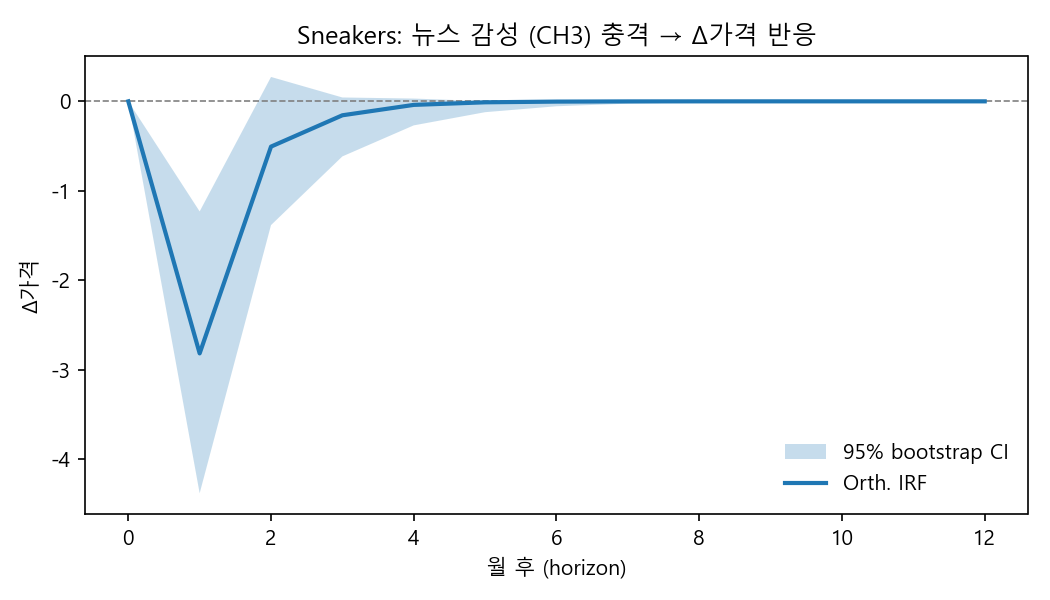
\includegraphics[width=0.48\textwidth]{../results/figures/irf_sneakers_ch3.png}\hfill
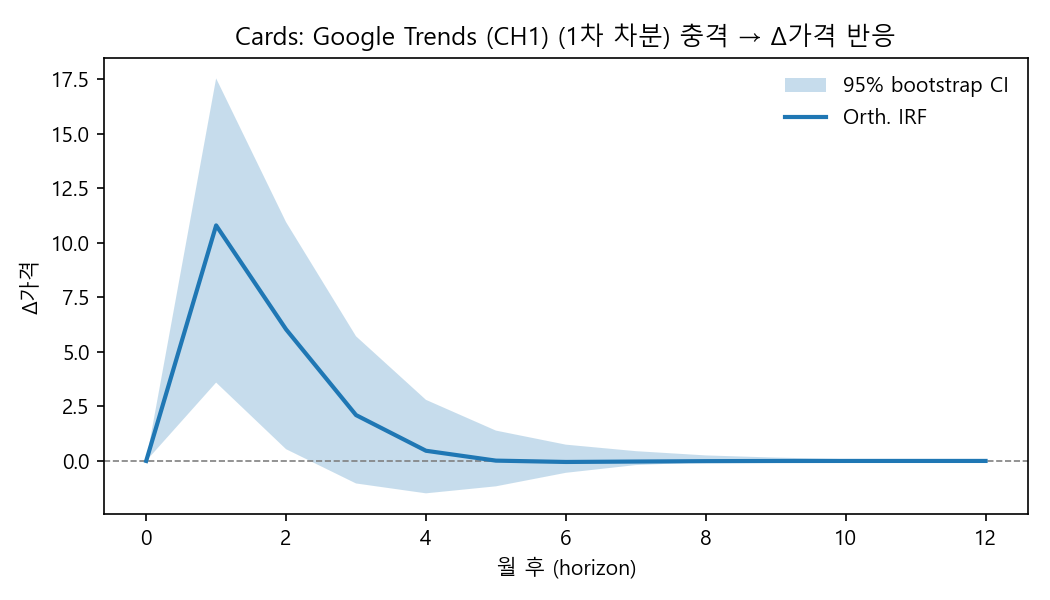
\includegraphics[width=0.48\textwidth]{../results/figures/irf_cards_ch1.png}
\caption{BH 보정 후 유의 채널에 대한 직교화 충격반응함수(95\% 잔차
부트스트랩 신뢰구간). \textbf{왼쪽:} sneakers의 뉴스 감성(CH3) 1 표준편차
충격에 대한 차분 가격($\Delta P_t$)의 12개월 반응. 1개월 시점에 $-2.82$
(CI $[-4.38,\ -1.23]$)로 가장 큰 음의 반응을 보이며 4개월 내 0으로
감쇄한다. \textbf{오른쪽:} cards의 Google Trends(CH1) 1차 차분 충격에 대한
차분 가격의 반응. 1\textasciitilde2개월에서 양의 반응이 유의하며($+10.80$,
$+6.03$, 두 CI 모두 0을 포함하지 않음), 3개월 이후 빠르게 감쇄한다.
횡축은 충격 후 경과 월, 음영은 95\% 부트스트랩 신뢰구간이다.}
\label{fig:irf}
\end{figure*}

\textbf{결과.} 그림 \ref{fig:irf}는 두 충격반응 패턴이 모두 \emph{단기
선행 + 빠른 감쇄}라는 공통 구조를 보임을 나타낸다. 동시에 부호의 방향은
자산-채널 조합에 따라 정반대로 나타난다.

\emph{cards--CH1.} Google Trends 1 SD 상승 시 1개월 후 가격 차분이 $+10.80$
달러(CI $[+3.59,\ +17.55]$), 2개월 후 $+6.03$ (CI $[+0.54,\ +10.95]$)로
유의한 양의 반응을 보인다. 이는 \citet{daengelberggao2011}의 ``검색
관심 → 단기 가격 상승 압력'' 패턴과 부호가 일치하며, 트레이딩 카드 시장에서
검색 관심도가 매수 수요의 선행 지표로 기능할 수 있음을 시사한다.

\emph{sneakers--CH3.} 뉴스 감성 1 SD 상승 시 1개월 후 가격 차분이 $-2.82$
달러(CI $[-4.38,\ -1.23]$)로 유의한 \emph{음}의 반응을 보인다. Granger
검정은 부호를 식별하지 않으므로 본 음의 부호는 IRF에서 처음 드러난
결과이다. 이는 다음 두 경로로 해석 가능하다. 첫째, 긍정 뉴스가 종종
\emph{공식 재발매·콜라보 발표}와 동시에 발생하는데, 이러한 발표는 신규
공급 신호로 작용하여 리셀 프리미엄을 단기적으로 압축할 수 있다(공급 충격
경로). 둘째, GDELT 톤은 도메인 특화 어휘(스니커즈 ``hype'', ``GR'') 대신
일반 뉴스 어휘의 감성을 측정하므로, 측정 노이즈가 부호에 영향을 줄
가능성도 배제할 수 없다(\S\ref{sec:discussion-limit} 참조). 두 경로 중
어느 것이 우세한지는 본 표본만으로는 식별 불가하며, 향후 도메인 특화
사전 또는 발표 이벤트 더미와의 결합 분석이 필요하다.

\textbf{공통 패턴.} 두 채널 모두 \emph{1\textasciitilde2개월 선행 + 4개월
내 소멸}의 단기 충격 구조를 보인다. 이는 미디어 신호가 \emph{지속적}
가격 추세보다는 \emph{국지적} 수급 충격으로 작용한다는 해석과 부합하며,
\S\ref{sec:results-rq3}의 RQ3 결과(전 채널 모형 대비 절제된 우수성)와도
일관된다.

\subsection{RQ2: 자산별 유의 채널 구성 비교}\label{sec:results-rq2}

SIGNIFICANT 판정 채널만을 자산별 유의 채널 집합으로 정의하면 다음과 같다.
\begin{itemize}[leftmargin=1.4em, topsep=2pt, itemsep=1pt]
  \item 스니커즈: $S_{\text{sneakers}} = \{\text{CH1, CH3, CH4}\}$
  \item 카드: $S_{\text{cards}} = \{\text{CH1}\}$
  \item 레고: $S_{\text{lego}} = \emptyset$
\end{itemize}

세 자산쌍의 Jaccard 유사도는 표 \ref{tab:jaccard}와 같다.

\begin{table*}[!tbp]
\centering\small
\caption[자산쌍별 Jaccard 유사도]{\textbf{세 자산쌍의 Jaccard 유사도
$J(S_a, S_b) = |S_a \cap S_b| / |S_a \cup S_b|$.} $S_a$는 자산 $a$의
\emph{SIGNIFICANT 판정 채널 집합}이며, MARGINAL 채널은 RQ2의 보수적
판정을 위해 본 집합 정의에서 제외된다(자세한 정의는
\S\ref{sec:method-jaccard} 참조). 본 연구의 임계는 $J<0.3$이면 ``자산별
채널 구성이 다름''(RQ2 지지), $0.3 \leq J \leq 0.6$이면 ``부분적 차이'',
$J>0.6$이면 ``구성 유사''로 판정한다. sneakers--cards 쌍은 $J=0.333$
으로 ``부분적 차이'' 구간에 속하며 두 자산이 CH1(Google Trends)을
공통 선행 채널로 공유함을 의미한다. sneakers--lego와 cards--lego
쌍은 lego가 SIGNIFICANT 채널을 갖지 않아 $J=0.000$으로 산출되며, 이는
``완전한 이질성''으로 해석된다.}
\label{tab:jaccard}
\begin{tabular}{llc}
\toprule
자산쌍 & 비교 집합 & $J$ \\
\midrule
sneakers -- cards & $\{\text{CH1,CH3,CH4}\}$ vs $\{\text{CH1}\}$ & $0.333$ \\
sneakers -- lego  & $\{\text{CH1,CH3,CH4}\}$ vs $\emptyset$       & $0.000$ \\
cards -- lego     & $\{\text{CH1}\}$ vs $\emptyset$               & $0.000$ \\
\bottomrule
\end{tabular}
\end{table*}

세 자산쌍 중 sneakers--cards는 $J = 0.333$으로 방법론 절의
``부분적 차이''($0.3 \leq J \leq 0.6$) 구간에 속하며, 두 자산이 모두
CH1(Google Trends)에서 선행성을 공유한다. 나머지 두 자산쌍은 $J=0.000$
으로 완전히 이질적이다.

\noindent\textbf{RQ2 결론:} 미디어 채널의 유의 구성은 자산 유형 간에
대체로 상이하며, 특히 레고는 다른 두 자산과 공통 채널을 공유하지
않는다. 단, sneakers와 cards는 CH1(Google Trends)을 공통 선행 채널로
가져 부분적 중복이 존재한다. 따라서 RQ2는 \emph{대체로 지지}되되,
검색 트렌드(CH1)는 자산 간 공통적 선행 신호일 가능성이 있다.

\subsection{RQ3: XGBoost 예측 검증 및 Diebold--Mariano 검정}
\label{sec:results-rq3}

Model A(전채널)와 Model B(Granger 선별 채널)를 \texttt{TimeSeriesSplit}
($n_{\text{splits}}=4$, \texttt{test\_size}$=6$)으로 학습하고, 4개
폴드 전체의 예측 오차를 합산하여($T=24$/아이템) Diebold--Mariano
검정을 수행하였다.\footnote{예측 대상은 월별 평균 가격(\textsf{mean\_price},
회귀)이며, 손실함수는 제곱오차($h=1$, Newey--West 추정)를 사용하였다.}
결과는 표 \ref{tab:dm}와 같다.

\begin{table*}[!tbp]
\centering\small
\caption[Diebold--Mariano 검정 결과]{\textbf{아이템별
Diebold--Mariano(DM) 검정 결과: Model A (전 채널) vs.\ Model B
(Granger 선별 채널).} 각 아이템에 대해 \texttt{TimeSeriesSplit}
($n_{\text{splits}}=4$, \texttt{test\_size}$=6$)으로 4개 폴드의 예측
오차를 합산하여 $T=24$개 시점에 대해 DM 검정을 수행하였다. 예측
대상은 월별 평균 가격(\textsf{mean\_price}, 회귀)이며, 손실 함수는
제곱오차($h=1$, Newey--West 추정)이다. DM 통계량이 음(陰)이면 Model A의
오차가 Model B 대비 작음을(Model A 우수), 양(陽)이면 Model B의 오차가
작음을(Model B 우수) 의미한다. 본 연구의 RQ3 판정 기준은 $p<0.05$
이고 부호가 Model B에 유리한 경우를 ``RQ3 지지''로, $p>0.10$인
경우를 ``간결성 확보(통계적 등가)''로, $0.05\leq p<0.10$인 경우를
``경계 수준''으로 보고한다. 15개 아이템 중 11개(73\%)에서 통계적으로
유의한 차이가 관찰되지 않았으며, sneakers\_jordan1($p<0.001$)과
lego\_falcon($p=0.032$)에서만 Model A가 유의하게 우수하였다.
sneakers\_nb550($p=0.062$)은 경계 수준에서 Model B가 우세인 유일한
사례이다.}
\label{tab:dm}
\begin{tabular}{llrrl}
\toprule
자산 & 아이템 & DM 통계량 & $p$ & 판정 \\
\midrule
\multirow{5}{*}{sneakers}
 & sneakers\_jordan1 & $-4.29$ & $<0.001$ & \textbf{Model A 우수} \\
 & sneakers\_panda   & $-1.47$ & $0.155$  & 차이 없음 \\
 & sneakers\_yeezy   & $-1.09$ & $0.288$  & 차이 없음 \\
 & sneakers\_travis  & $\phantom{-}0.38$ & $0.705$ & 차이 없음 \\
 & sneakers\_nb550   & $\phantom{-}1.96$ & $0.062$ & Model B 우세(경계) \\
\midrule
\multirow{5}{*}{cards}
 & cards\_charizard1 & $\phantom{-}1.23$ & $0.230$ & 차이 없음 \\
 & cards\_charizard2 & $\phantom{-}1.49$ & $0.150$ & 차이 없음 \\
 & cards\_umbreon    & $-0.56$ & $0.580$  & 차이 없음 \\
 & cards\_rayquaza   & $-0.02$ & $0.985$  & 차이 없음 \\
 & cards\_pikachu    & $\phantom{-}0.38$ & $0.711$ & 차이 없음 \\
\midrule
\multirow{5}{*}{lego}
 & lego\_falcon      & $-2.28$ & $0.032$  & \textbf{Model A 우수} \\
 & lego\_hogwarts    & $\phantom{-}1.27$ & $0.217$ & 차이 없음 \\
 & lego\_titanic     & $-0.56$ & $0.579$  & 차이 없음 \\
 & lego\_porsche     & $-1.75$ & $0.094$  & Model A 우세(경계) \\
 & lego\_bugatti     & $\phantom{-}0.42$ & $0.677$ & 차이 없음 \\
\midrule
\multicolumn{5}{l}{\textit{주.} DM 통계량 $> 0$이면 Model B의 오차가 작음(B 우수).
  $p < 0.05$ 유의, $p < 0.10$ 경계.}
\end{tabular}
\end{table*}

15개 아이템 중 11개(73\%)에서 Model A와 B 간 통계적으로 유의한 차이가
관찰되지 않았다. \textsf{sneakers\_jordan1}($p<0.001$)과
\textsf{lego\_falcon}($p=0.032$)에서는 Model A가 유의하게 우수하였으며,
\textsf{lego\_porsche}($p=0.094$)는 경계 수준에서 Model A가 우세하였다.
반면 \textsf{sneakers\_nb550}($p=0.062$)은 경계 수준에서 Model B가
우세하였다.

\begin{figure*}[!tbp]
\centering
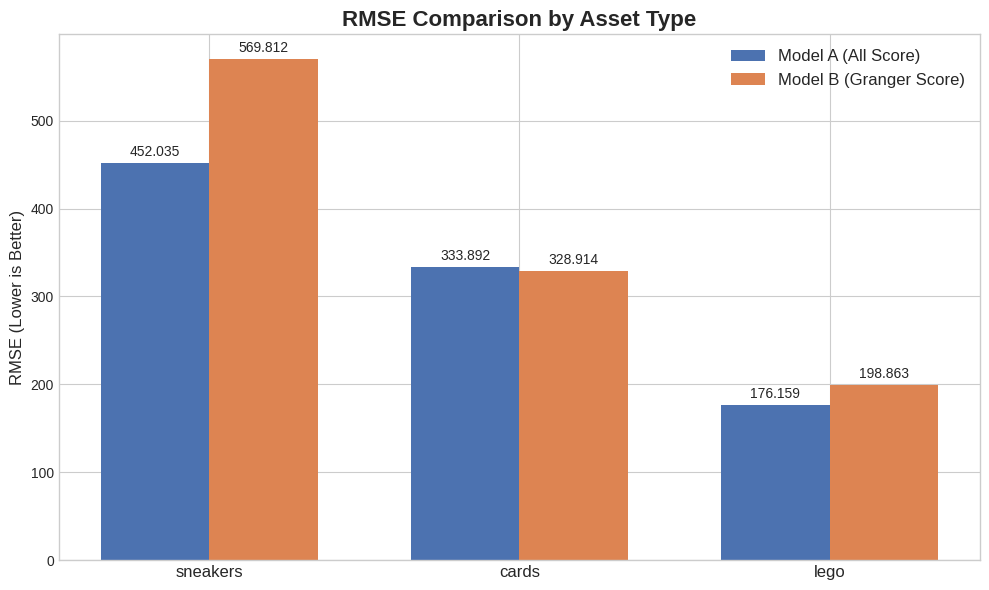
\includegraphics[width=0.72\textwidth]{../results/figures/reg_rmse_bar_00.png}
\caption[자산별 RMSE 비교]{\textbf{자산별 RMSE 비교: Model A(전 채널)
vs.\ Model B(Granger 선별 채널).} 가로축은 자산군별로 묶인 15개 아이템,
세로축은 \texttt{TimeSeriesSplit}($n_{\text{splits}}=4$,
\texttt{test\_size}$=6$)으로 산출한 4개 폴드 전체의 RMSE(Root Mean
Squared Error, 단위: USD)이다. 막대 높이가 낮을수록 예측 오차가
작아 모형의 정확도가 높음을 의미한다. 각 아이템에서 좌측 막대(짙은
색)는 통제 피처(\textsf{price\_vs\_ma3}, \textsf{price\_chg\_lag1\textasciitilde3})
와 CH1\textasciitilde CH5 전 채널을 사용하는 Model A의 RMSE이며,
우측 막대(밝은 색)는 통제 피처와 \emph{Granger 유의 또는 경계로
판정된 채널만}을 사용하는 Model B의 RMSE이다. 자산별 평균 RMSE를
살펴보면, sneakers는 Model A($452$) $<$ Model B($569$), lego는
Model A($176$) $<$ Model B($199$)로 Model A가 일관되게 낮은 반면,
cards는 두 모형이 사실상 동등하다(Model A $334$ vs.\ Model B $329$).
sneakers\_jordan1과 lego\_falcon에서 Model A와 B의 격차가 가장 크며,
이는 DM 검정(표~\ref{tab:dm})에서 두 아이템이 Model A 우수로 판정된
결과와 정합된다. 단, DM 검정의 ``차이 없음'' 판정과 자산 평균 RMSE의
일관된 격차는 동일한 결론을 지시하지 않는다 ─ 측정 대상의 차이는
\S\ref{sec:discussion-limit}에서 다룬다.}
\label{fig:rmse}
\end{figure*}

\textbf{RMSE 평균과 DM 등가성의 괴리.} 그림 \ref{fig:rmse}의 자산별
평균 RMSE는 sneakers에서 Model A($452$) vs.\ Model B($569$), lego에서
Model A($176$) vs.\ Model B($199$)로 Model A가 일관되게 낮다. cards에서만
양 모형이 사실상 동등하다($334$ vs.\ $329$). 이는 DM 검정의 ``차이
없음'' 판정과 일견 충돌하나, 두 지표는 측정 대상이 다르다. DM 검정은
폴드 합산 시계열 예측 오차의 \emph{시점별 부호 차이}를 자기상관 보정
후 평가하는 반면, RMSE 평균은 절대 오차의 산술 평균이므로 일부 큰
오차에 강하게 영향받는다. 두 지표의 비대칭성은
\S\ref{sec:discussion-limit}에서 한계로 다룬다.

\noindent\textbf{RQ3 결론(절제된 해석):} DM 검정 기준 15개 아이템 중
11개(73\%)에서 Model A와 Model B 간 통계적으로 유의한 예측 오차 차이가
관찰되지 않았다. 그러나 자산별 평균 RMSE는 sneakers와 lego에서 Model A가
일관되게 낮으며, Model A가 유의하게 우수한 2개 아이템(\textsf{jordan1},
\textsf{falcon})이 존재한다. 따라서 본 결과는 ``Model B가 Model A보다
우수하다''는 적극적 결론이 아니라, \emph{Granger 선별이 다수 아이템에서
큰 정보 손실 없이 채널 수를 축소할 수 있는 도구일 수 있음}을 시사하는
\emph{절제된} 발견으로 해석되어야 한다. 자세한 한계는 논의 절에서 다룬다.

\subsubsection*{하이퍼파라미터 튜닝에 대한 견고성 검토}
\label{sec:results-tuning}

본 절의 주 분석은 고정 하이퍼파라미터(\texttt{n\_estimators}=100,
\texttt{max\_depth}=3, \texttt{learning\_rate}=0.05)를 사용한다. 두 모형
모두 동일 설정을 적용하여 비교 공정성을 유지하였으나, ``Model A가 더
큰 피처 공간을 활용하므로 튜닝되지 않은 default에 우연히 더 잘 맞았을
가능성''이 잠재한다. 본 절은 이 가능성을 통제하기 위해 Optuna
TPE\citep{akibasanouama2019} 기반 60회 베이지안 최적화를 자산별
$\times$ 모형별로 독립 수행하여(총 $60\times 3\times 3 = 540$ trial),
튜닝된 조건에서 동일 DM 검정을 재실행한다.\footnote{탐색 공간:
\texttt{n\_estimators} $\in [50,300]$, \texttt{max\_depth} $\in [2,6]$,
\texttt{learning\_rate} $\in [0.01,0.2]$ (log), \texttt{subsample}/
\texttt{colsample\_bytree} $\in [0.6,1.0]$, \texttt{min\_child\_weight}
$\in [1,5]$, \texttt{reg\_lambda} $\in [0,5]$, \texttt{reg\_alpha} $\in [0,1]$.
TimeSeriesSplit($n=4$, test\_size=6)으로 자산 내 모든 아이템 평균 RMSE를
최소화. 동일 절차로 \emph{Model B-DH}(\S\ref{sec:results-dh}의 DH 검정
유의 채널 사용)도 추가 비교에 포함하였다.} 결과는 표
\ref{tab:tuned}와 같다.

\begin{table}[!t]
\centering\small
\caption[XGBoost 튜닝 후 DM 결과]{\textbf{Optuna 튜닝 후 자산별 평균
RMSE 및 DM 판정 분포.} ``기존''은 고정 하이퍼파라미터 결과(표
\ref{tab:dm}), ``튜닝''은 자산$\times$모형별 60회 베이지안 최적화 후
결과. \textit{B-DH}는 \S\ref{sec:results-dh}의 DH 검정 결과를 반영한
선별 채널 모형이며, lego는 DH에서 모든 채널이 비유의이므로 통제 피처
4개만을 사용한다(채널 0개). 튜닝 후 절대 RMSE 수치는 크게 감소하지만
세 모형 간 \emph{상대적 순위}는 유지된다: 모든 자산에서 Model A의 RMSE가
가장 낮으며, sneakers와 lego에서 양의 격차가 일관된다.}
\label{tab:tuned}
\begin{tabular}{lrrr}
\toprule
자산 & A (RMSE) & B-original & B-DH \\
\midrule
sneakers & \textbf{61.14} & 73.19 & 76.14 \\
cards    & \textbf{194.04} & 194.29 & 194.69 \\
lego     & \textbf{40.45} & 44.44 & 43.41 \\
\midrule
\multicolumn{4}{l}{\textit{DM 판정 분포 (A vs B-original, $n=15$)}} \\
구분 & 기존 & 튜닝 후 & \\
\midrule
차이 없음 & 11 & 10 & \\
Model A 우수 & 2 & \textbf{5} & \\
Model B 경계 우세 & 1 & 0 & \\
Model A 경계 우세 & 1 & 0 & \\
\bottomrule
\end{tabular}
\end{table}

표 \ref{tab:tuned}에서 두 가지 관찰이 도출된다. 첫째, 튜닝은 두 모형의
절대 RMSE를 모두 크게 낮추지만(sneakers Model A: 452 $\rightarrow$ 61,
lego Model A: 176 $\rightarrow$ 40), \emph{모형 간 상대 순위는 유지}된다.
이는 주 분석의 ``Model A 일관 우세''결론이 단순 default 적합의 부산물이
아님을 시사한다. 둘째, DM 검정에서 ``Model A 우수''로 판정되는 아이템은
2개에서 5개로 증가하고(\textsf{yeezy}, \textsf{charizard1},
\textsf{porsche} 추가), ``Model B 경계 우세''(\textsf{nb550})는 사라진다.
즉 튜닝 후에는 Model A 우월성이 약간 더 명확하다. 그럼에도 \emph{차이
없음} 비율은 67\%(10/15)로 여전히 다수이므로, \S\ref{sec:results-rq3}의
``절제된 결론''은 유지된다.

\emph{B-DH 모형}은 자산별 평균 RMSE에서 B-original과 유의한 차이가 없다
(아이템별 DM 검정: 15개 중 12개 ``차이 없음'', 1개 ``B-original 우수'',
2개 경계). DH 검정에서 cards에 CH2가 추가되고 lego에서는 채널이 제거되는
변화가 \emph{예측 성능}에는 거의 반영되지 않는다는 사실은, Granger
선별(통계적 인과성)과 비선형 예측력(SHAP 기여도) 간의 비대칭성을 다시
한 번 시사한다(\S\ref{sec:discussion-shapgranger} 참조). 본 견고성 검토
스크립트는 \texttt{scripts/tune\_xgboost.py}에, 결과는
\texttt{results/xgboost\_tuned\_params.csv}, \texttt{results/xgboost\_tuned\_rmse.csv},
\texttt{results/dm\_tuned.csv}에 보존되어 있다.

% =====================================================================
\section{논의}\label{sec:discussion}

\subsection{채널별 선행성의 자산별 분화}\label{sec:discussion-rq12}

Granger 검정 결과는 미디어 채널의 선행적 역할이 자산 유형에 따라 분화될
\emph{잠정적} 가능성을 시사한다. 스니커즈에서는 Google Trends(CH1),
뉴스 감성(CH3), YouTube 조회수(CH4) 세 채널이 유의 수준에서 선행성을
보였다. CH3의 $F$ 통계량(13.38)이 15회 검정 중 가장 컸으나, 표본 크기와
다중 검정 구조를 고려하면 이를 단정적 인과 증거로 해석하는 데는 신중함이
요구된다. 스니커즈 리셀 시장이 출시 전후 미디어 보도와 셀럽 협업 소식에
민감하게 반응하는 특성을 가진다는 점에서, 본 결과는 해당 자산의 정보
생성 메커니즘과 정합되는 방향으로 읽힐 수 있다.

카드 시장에서는 Google Trends(CH1, $F=8.42$)가 유의 수준에서 선행하였다.
이는 트레이딩 카드 수요가 커뮤니티 내 검색 관심도와 연동될 가능성을 시사하나,
인과 메커니즘의 확정에는 추가 연구가 필요하다. 레고에서는 CH1이 경계
수준에 그쳐 명확한 선행 채널이 관찰되지 않았으며, 이는 레고 단종 세트의
가격이 미디어 채널보다 재고 수급과 공급 측 정보에 더 강하게 의존할
가능성을 함의한다.

\subsection{Granger 선행성과 XGBoost SHAP 기여도의 관계}
\label{sec:discussion-shapgranger}

Granger $F$ 순위와 XGBoost SHAP 순위 간에는 체계적 불일치가 관찰된다
(표 \ref{tab:shap}). 스니커즈에서 Granger $F$ 1위인 CH3(뉴스 감성)의
평균 $|\text{SHAP}|$는 0.011로 채널 5개 중 최하위에 해당하며, Granger
비유의인 CH5(0.124)와 Granger $F$ 3위인 CH1(0.125)이 SHAP 기여도
최상위를 차지한다.

\begin{table*}[!tbp]
\centering\small
\caption[채널별 평균 $|\text{SHAP}|$]{\textbf{Model A 분류기에서 산출한
채널별 평균 $|\text{SHAP}|$ 값과 Granger 판정의 비교.} $|\text{SHAP}|$는
SHAP 값의 절댓값을 의미하며, 행 평균은 해당 채널이 \emph{모든 관측에
걸쳐 모형 예측에 미친 평균적 한계 기여도}로 해석된다(``전역 변수
중요도''). 동일 행의 ``Granger 판정''은 표~\ref{tab:granger}의 결과로,
SIG는 SIGNIFICANT, MARGINAL은 MARGINAL, NOT은 NOT\_SIG을 의미한다.
sneakers에서 Granger $F$ 1위인 CH3는 $|\overline{\text{SHAP}}|=0.011$
로 채널 중 최하위에 해당하며, Granger 비유의인 CH5(0.124)와 CH1(0.125)
이 SHAP 상위를 차지하여 \emph{선형 인과성과 비선형 예측 기여의 측정
대상이 다름}을 직접적으로 드러낸다. cards와 lego에서는 CH4가 SHAP
1위이나 Granger에서는 비유의여서, 채널 단독 Granger 검정이 비선형
신호를 포착하지 못하는 한계를 시사한다. 본 표의 자세한 해석은
\S\ref{sec:discussion-shapgranger}에서 다룬다.}
\label{tab:shap}
\begin{tabular}{llrrrrr}
\toprule
자산 & & CH1 & CH2 & CH3 & CH4 & CH5 \\
\midrule
sneakers & $|\overline{\text{SHAP}}|$ & 0.125 & 0.000 & 0.011 & 0.080 & 0.124 \\
         & Granger 판정 & \textbf{SIG} & NOT & \textbf{SIG} & \textbf{SIG} & NOT \\
\midrule
cards    & $|\overline{\text{SHAP}}|$ & 0.048 & 0.031 & 0.025 & 0.091 & 0.004 \\
         & Granger 판정 & \textbf{SIG} & NOT & NOT & NOT & NOT \\
\midrule
lego     & $|\overline{\text{SHAP}}|$ & 0.036 & 0.003 & 0.000 & 0.070 & 0.021 \\
         & Granger 판정 & MARGINAL & NOT & NOT & NOT & NOT \\
\bottomrule
\multicolumn{7}{l}{\textit{주.} SIG = SIGNIFICANT, MARGINAL = MARGINAL, NOT = NOT\_SIG.}
\end{tabular}
\end{table*}

이 불일치는 두 방법의 측정 대상이 근본적으로 다른 데서 기인한다.
Granger 검정은 \emph{채널 단독으로, 가격의 과거값만 통제한 상태}에서
해당 채널이 선형적으로 선행하는지를 평가한다. 반면 SHAP은
\emph{모든 변수가 동시에 투입된 비선형 모형에서 채널의 한계 기여도}를
측정한다. 가격 모멘텀 변수(\textsf{price\_vs\_ma3}, \textsf{price\_chg\_lag1})가
예측 분산의 대부분을 흡수한 이후에는, Granger에서 선행성을 보인 채널이라
하더라도 XGBoost 내에서 추가로 기여할 분산이 제한적이다. CH3(뉴스 감성)와
같이 선형적 선행성이 강한 채널이 가격 모멘텀과 높은 공분산을 갖는 경우,
가격 라그 변수가 해당 채널의 신호를 미리 포착하여 SHAP 기여도를 잠식한다.

\begin{figure*}[!tbp]
\centering
\includegraphics[width=\textwidth, height=0.27\textheight, keepaspectratio]%
  {../results/figures/clf_shap_asset_00.png}\\[4pt]
\includegraphics[width=\textwidth, height=0.27\textheight, keepaspectratio]%
  {../results/figures/clf_shap_asset_02.png}\\[4pt]
\includegraphics[width=\textwidth, height=0.27\textheight, keepaspectratio]%
  {../results/figures/clf_shap_asset_04.png}
\caption[자산별 XGBoost 피처 중요도 및 SHAP Summary Plot]{\textbf{자산별
XGBoost 피처 중요도 및 SHAP Summary Plot (Model A, 분류 기준).} 각
행은 자산군 한 곳에 대응하며, 위부터 차례로 스니커즈, 카드, 레고
이다. 각 행은 두 패널로 구성된다 ─ \textbf{왼쪽 패널}은 XGBoost의
\emph{Gain 기반 피처 중요도}로, 각 변수가 트리 분기점으로 선택될
때 발생시킨 손실 함수 감소량의 누적값에 비례한다(클수록 모형 내
중요도가 큼). \textbf{오른쪽 패널}은 SHAP Summary Plot으로, 점 하나가
하나의 관측 월(아이템--월)을 나타내며, 점의 가로 좌표는 해당 관측에
대한 변수의 SHAP 값(예측 logit에의 기여 부호와 크기), 점의 색은
해당 관측에서의 \emph{변수값 자체}(붉을수록 높은 값, 푸를수록 낮은
값)를 표현한다. 변수는 평균 $|\text{SHAP}|$ 내림차순으로 정렬되어
있으며, 통제 피처(\textsf{price\_vs\_ma3}, \textsf{price\_chg\_lag1
\textasciitilde 3})가 모든 자산에서 상위를 차지한다. 채널 변수만을
보면, sneakers는 CH1·CH5가 채널 중 상위 두 자리를 점유하고 Granger
$F$ 1위였던 CH3는 채널 최하위로 떨어진다. cards는 CH4가 채널 1위,
CH1이 2위이며, lego도 CH4가 채널 1위, CH1이 2위로 cards와 유사한
구조이다. 이 결과는 표~\ref{tab:shap}의 수치적 정리와 일관되며,
선형 인과성(Granger)과 비선형 예측 기여(SHAP)의 측정 대상이
근본적으로 다름을 시각적으로 보여 준다(\S\ref{sec:discussion-shapgranger}
참조).}
\label{fig:shap_asset}
\end{figure*}

이 결과는 통계적 인과성(Granger)과 예측적 기여도(SHAP)가 동일한 개념이
아님을 보여 주며, 두 지표를 함께 보고함으로써 채널의 역할을 다각도로
해석할 수 있다는 점에서 방법론적 기여가 있다.

\subsection{Model A 우수 예외 아이템 분석}
\label{sec:discussion-exceptions}

\textsf{sneakers\_jordan1}과 \textsf{lego\_falcon}에서는 Model A가
통계적으로 유의하게 우수하였다. 두 아이템 모두 해당 자산군의 대표적
플래그십 제품으로, 미디어 채널의 영향이 단일 채널을 초과하는 다층적
구조를 가질 가능성이 있다.

스니커즈 Model B는 Granger 유의 채널인 CH3와 CH4만을 포함하나, SHAP
분석에 따르면 CH1(0.125)과 CH5(0.124)가 채널 기여도 상위를 차지한다.
즉 \textsf{jordan1}의 예측에서 실질적으로 중요한 채널은 Granger로
선별되지 않은 채널이었으며, 이로 인해 Model B가 정보 손실을 겪었다.

\textsf{lego\_falcon}의 경우 레고 Model B는 CH1만을 포함하지만, SHAP
분석에서 CH4(0.070)가 CH1(0.036)보다 높은 기여도를 보인다. Millennium
Falcon은 Star Wars 관련 이벤트와 연동된 YouTube 콘텐츠 급증이 주기적으로
발생하는 아이템으로, 채널 단독 Granger 검정이 CH4의 복잡한 비선형 기여를
포착하지 못한 결과로 해석된다.

두 사례는 Granger 선별이 특정 아이템에서는 최적 채널 집합을 과소 포함할
수 있음을 보여 주며, 이를 한계로 명시한다.

\subsection{한계}\label{sec:discussion-limit}

본 연구의 한계는 다음과 같다.

\textbf{소표본 및 다중 검정의 검정력 제약.} 자산당 48개월의 관측치는
Granger 검정과 XGBoost 교차검증 모두에서 통계적 검정력을 제약한다.
래그 1--4 범위에서 BIC로 래그를 선택하더라도 유효 관측치는 44--47개로
감소하며, 동일 자산에 대해 5개 채널을 순차적으로 검정하므로 자유도
압박과 다중 비교 문제가 누적된다. 본 연구가 결과를 \emph{탐색적}
발견으로 명시하고 BH 보정 결과를 부록에 함께 제시하는 것은 이러한
구조적 한계를 보완하기 위함이며, 본 결과를 확증적(confirmatory) 증거로
일반화하기 위해서는 더 긴 패널과 사전 등록 설계가 요구된다.

\textbf{ADF 정상성의 한계.} sneakers의 \textsf{score\_ch1}은 1차 차분
후에도 ADF $p=0.120$으로 단위근을 엄밀히 기각하지 못한다(표
\ref{tab:stationarity} 각주 †). 실질적 자기상관 감소를 근거로 차분값을
Granger 검정에 투입하였으나, 비정상 잔차가 잔존할 경우 sneakers CH1
($p=0.041$)의 SIGNIFICANT 판정이 약화될 수 있다. 본 채널은 BH 보정
시에도 NOT\_SIG로 탈락한다는 점에서 견고성이 가장 약한 발견이며,
후속 연구에서 KPSS 추가 검토와 더 긴 패널을 통한 재현이 필요하다.

\textbf{분석 단위 불일치(자산 수준 Granger vs.\ 아이템 수준 XGBoost).}
RQ1·RQ2의 Granger 검정은 아이템 5개의 월별 평균을 사용한 \emph{자산-월
단위 대표 시계열}에서 수행되며, RQ3의 XGBoost/DM은 15개 \emph{아이템-월
단위}에서 수행된다. Model B의 채널 구성은 \emph{자산 수준 Granger
결과}를 동일 자산군의 모든 아이템에 일률적으로 적용하므로, 개별 아이템
수준에서는 다른 채널이 더 적합할 수 있다(예: \textsf{lego\_falcon}에서
SHAP CH4가 CH1보다 큼; \S\ref{sec:discussion-exceptions}). 자산 수준
평균은 아이템 간 잡음 감쇄 효과가 있으나, 단위 정합성 측면에서는
패널 VAR\citep{holtzeakinneweyrosen1988}이나 이질적 패널 Granger
검정\citep{dumitrescuhurlin2012} 또는 아이템별 단독 Granger 설계가
더 엄밀하다. 본 연구는 \S\ref{sec:results-dh}에서 DH 패널 Granger를,
\S\ref{sec:results-var}에서 다변수 VAR 블록·개별 인과 검정을
보충 적용하여 이 한계를 \emph{부분적으로} 해소하였으며, BH 보정 후
세 검정 모두에서 일관 유의한 채널이 cards--CH1로 집약됨을 확인하였다.
추가로 \S\ref{sec:results-var}의 다변수 VAR 블록·개별 검정은 채널 간
다중공선성을 통제한 후에도 cards--CH1과 sneakers--CH3가 BH 보정을
통과함을 보여, 세 검정의 교집합 발견(cards--CH1)을 자산-공통의 가장
견고한 미디어 선행 채널로 확립한다(표 \ref{tab:three_tests}).
그러나 본 검정은 $N=5$로 정규 근사가 비교적 약하고 표준 점근
근사만을 사용하였으므로, 잔차 부트스트랩 변형의 적용은 후속 과제로
남는다.

\textbf{CH3 대리변수.} 뉴스 감성(CH3)은 NewsAPI+FinBERT를 원설계로 하였으나,
무료 플랜의 역사 자료 30일 제한으로 GDELT \texttt{timelinetone}으로 대체하였다.
GDELT 톤은 도메인 특화 학습 없이 자동 산출되는 일반 감성 점수로, 리셀
특화 어휘·맥락에 대한 감도가 낮을 수 있다.

\textbf{sneakers\_yeezy 결측.} StockX 거래량 표본 추출 아티팩트로 4개월
결측이 발생하여 선형 보간으로 처리하였다. 보간 구간의 가격 변동이 비선형
이었을 경우 분석 결과에 편의를 유발할 수 있다.

\textbf{lego\_porsche·bugatti Google Trends 0값.} 해당 아이템의 CH1
점수에는 각각 21/48, 25/48개월의 0값이 포함되어, 채널 신호의 정보량이
제한된다. 이는 CH1 관련 분석에서 과소 추정 편의를 유발할 수 있으며,
결과 해석 시 유의해야 한다.

\textbf{z-score 전역 적합.} 채널 점수의 z-score는 전체 샘플로 추정하였다.
엄밀한 시계열 교차검증에서는 각 학습 폴드의 통계량만을 사용해야 하나,
소표본 특성상 폴드별 추정 분산이 커 전역 적합을 채택하였다. 이는 미미한
수준의 정보 누설 가능성을 내포한다.

\textbf{DM 검정의 태스크 불일치.} 메인 XGBoost는 가격 방향성(0/1, 분류)을
예측하나, DM 검정은 평균 가격 수준(회귀, RMSE 기반)의 예측 오차를 비교한다.
두 태스크의 목적이 상이하므로 DM 결과를 분류 성능의 직접 증거로 해석하는
데는 한계가 있다. 마찬가지로 표 \ref{tab:shap}의 SHAP 분석은 \emph{분류
모형}에서 산출하므로, 표 \ref{tab:dm}의 \emph{회귀 기반 DM} 결과와
같은 적합 모형이 아니다. 두 결과는 동일 \emph{피처 집합} 하 보완 지표로
제시되며, 단일 모형 기반 일관 비교가 아님을 명시한다.

\textbf{RMSE 평균과 DM 등가성의 괴리.} \S\ref{sec:results-rq3}에서
보고하였듯, 자산별 평균 RMSE는 sneakers·lego에서 Model A가 일관되게
낮음에도 DM 검정은 ``차이 없음''으로 판정한 아이템이 대다수이다. 이는
DM이 \emph{시점별 오차 차이의 표본 평균}을 자기상관 보정 표준오차로
검정하므로 일부 큰 오차의 영향이 평균화되기 때문이다. 따라서 ``DM에서
유의한 차이가 없다''와 ``선별 채널이 우수하다''는 동치가 아니며, 실무적
권고는 평균 RMSE와 DM을 함께 보고하는 것이다. SPA(superior predictive
ability; \citealp{hansen2005}) 또는 MCS(model confidence set;
\citealp{hansenlundenason2011})와 같은 다중 모형 비교 절차를 적용한
후속 검증이 권장된다. 또한 추정 매개변수 불확실성을 반영한
\citet{west1996}의 예측 능력 추론은 DM의 보완 도구로 활용 가능하다.

\textbf{탐색적 연구 특성.} 본 연구는 리셀 시장에서의 미디어 채널 선행성을
처음으로 다중 자산·다중 채널 설계로 탐색하는 성격을 갖는다. 다중비교
보정(Benjamini--Hochberg FDR) 적용 시 sneakers CH1과 CH4가 자산-평균
유의 채널에서 탈락하여 유의 채널은 2개(sneakers CH3, cards CH1)로
줄어든다. \S\ref{sec:results-dh}의 DH 패널 검정에 동일 BH 보정을
적용하면 \emph{sneakers CH4, cards CH1}이 유지되어, 두 검정에서 BH
보정 후 일관되게 살아남는 발견은 \textbf{cards--CH1} 한 조합으로
좁혀진다. BH 보정 전후 결과 비교는 부록 표~\ref{tab:bh}에 제시한다.

\textbf{직접 선행 연구의 부재.} 본 연구는 리셀 시장 가격 결정에 미디어
채널 선행성을 다중 자산·다중 채널 설계로 비교한 거의 첫 시도로
보이며(\S\ref{sec:related} 참조), 이는 강점인 동시에 한계이다. 동일
정의·동일 기간에서 결과를 직접 비교 가능한 \emph{기준선(benchmark)}
연구가 부재하여, 본 연구의 효과 크기(예: sneakers CH3 $F=13.38$)가
리셀 시장 표준 분포 내 어느 위치에 있는지 평가할 수 없다. 본 발견은
향후 동일 설계의 반복 연구에서 견고성을 검증하는 출발점으로 활용될
필요가 있다.

\textbf{측정 범위의 한계 ─ 폐쇄형 SNS의 부재.} 본 연구의 다섯 채널은
\emph{공개 무료 API 또는 공개 웹 자료를 통해 일관되게 수집 가능한
채널}로 한정되었다. 따라서 Instagram·TikTok·Discord·Reddit 비공개
서브레딧과 같이 \emph{폐쇄형 또는 비공개 API}를 기반으로 하는 SNS는
분석에서 제외되었다. 이는 두 가지 측면에서 결과 해석에 영향을 미칠 수
있다. 첫째, 스니커즈·트레이딩 카드 커뮤니티의 상당 부분은 Discord
서버나 Instagram 마이크로 커뮤니티에서 정보 교환이 이루어지므로, 본
연구가 측정하지 못한 \emph{잠재적 선행 신호}가 존재할 가능성이 높다.
특히 TikTok의 짧은 영상 콘텐츠는 Z세대 수집가층의 정보 노출에 결정적
역할을 하나, 공개 API가 제한적이어서 시계열 수집이 어렵다. 둘째,
본 연구가 측정한 다섯 채널 중 일부(예: YouTube 조회수)가 통계적
선행성을 보였더라도, 이는 \emph{측정 가능한 채널 군 안에서의 상대적
효과}이며, 폐쇄형 채널까지 포함한 \emph{진정한 정보 환경}을 반영하지
는 못한다. 후속 연구는 (i) TikTok·Instagram Graph API의 공식 연구자
프로그램 신청, (ii) 사용자 동의 기반 Discord 데이터 수집, (iii)
Reddit Pushshift 아카이브 활용 등을 통해 채널 범위를 확장할 것을
권장한다.

\subsection{이론적 함의 ─ 자산별 채널 분화의 경제학적 해석}
\label{sec:discussion-theory}

본 연구의 핵심 발견 ─ 미디어 채널의 가격 선행성이 자산 유형별로 분화된다는 점 ─
은 단순한 통계적 패턴 이상의 함의를 가지며, 정보경제학과 행동재무학의
기존 이론적 프레임으로 해석될 수 있다. 본 절은 세 자산군에서 관찰된
이질적 채널 구성을 \emph{가격 형성의 정보 메커니즘 차이}로 환원하여
설명한다.

\textbf{스니커즈 ─ 정보 비대칭 해소 채널로서의 뉴스 감성.}
스니커즈에서 CH3(뉴스 감성)가 가장 강한 선행 효과($F=13.38$)를
보인 점은, 이 시장의 가격 결정이 \emph{출시 전후의 미디어 보도와
셀럽 협업 소식}에 강하게 의존한다는 점과 정합된다. 한정판 협업
출시 정보, 가품 적발, 셀럽 착용 사례 등은 \citet{tetlock2007}이 분석한
\emph{미디어 매개 정보 비대칭 해소} 메커니즘과 동일 구조를 가진다.
즉 보도의 \emph{양}이 아닌 \emph{방향}(부정/긍정 어조)이 가격 충격을
일으키며, 이는 \citet{tetlocksaarmacskassy2008}이 보고한 ``기업 펀더멘털
대비 부정 어휘의 추가 정보''와 정성적으로 부합한다. 본 결과는 \emph{스니커즈
시장의 가격 형성에서 미디어 보도가 인과적 기제(causal channel)로 작동할
가능성}을 시사하며, 이는 \citet{engelbergparsons2011}의 외생적 식별 전략을
리셀 시장으로 확장한 후속 연구로 발전 가능하다.

\textbf{트레이딩 카드 ─ 표준화된 등급제 하의 수요 신호.}
카드 시장에서 CH1(Google Trends)이 유일한 유의 채널인 점은, 본 시장의
\emph{정보 비대칭 수준이 상대적으로 낮다}는 구조적 특성에 기인한다고
해석할 수 있다. PSA 그레이딩은 카드의 품질 정보를 표준화함으로써 ``레몬
시장(market for lemons)'' 문제를 부분적으로 해소하므로, 신규 정보 충격이
상대적으로 드물고 가격은 \emph{잠재 수요의 변동}에 더 직접적으로 반응
한다. \citet{daengelberggao2011}의 검색 기반 관심 지표가 \emph{개별
자산의 수요 측 압력}을 측정한다는 직관과 일관되게, 카드 시장의 가격은
``뉴스보다 검색에 반응'' 한다는 패턴이 관찰된다. 이는 \citet{josephwintokizhang2011}이
보고한 ``검색 기반 비정상 수익률 예측'' 메커니즘과도 정합된다.

\textbf{레고 ─ 단종 후 공급 측 희소성의 우위.}
레고에서 어떤 미디어 채널도 명확한 선행 효과를 보이지 않은 점은
(CH1만 경계 수준), 본 시장이 \emph{공급 측 충격}에 강하게 의존한다는
사실을 시사한다. 단종된 레고 세트는 추가 생산이 불가능하므로 가격
형성의 핵심 변동 요인은 \emph{잔존 재고와 거래 빈도}이며, 이는
\citet{dobrynskayakishilova2022}이 보고한 ``LEGO 가격의 단종 후 평균
연 11\% 수익률''의 주된 메커니즘으로 알려져 있다. 즉 레고에서는
미디어 채널이 \emph{수요 신호}로서 작동하더라도 공급 측 비탄력성
때문에 가격에 매개되지 않는 셈이다. 본 해석은 \citet{burtonjacobsen1999}의
수집품 시장 분석에서 ``공급의 본질적 비탄력성''이 가격 변동성의
주된 동인이라는 결론과 부합한다.

\textbf{종합 ─ ``정보 비대칭 강도 $\times$ 공급 탄력성'' 2$\times$2 프레임.}
세 자산군의 채널 분화는 다음 두 차원의 결합으로 단순화될 수 있다.
(i) \emph{정보 비대칭 수준}: 스니커즈 高 vs.\ 카드 低 vs.\ 레고 中.
(ii) \emph{공급 탄력성}: 스니커즈 中(재출시 가능) vs.\ 카드 低(고정 발행량)
vs.\ 레고 極低(단종). 정보 비대칭이 높을수록 뉴스·감성 채널이 우월하며
(스니커즈 CH3), 비대칭이 낮으면 수요 신호인 검색 트렌드가 우월하다
(카드 CH1). 공급 탄력성이 극단적으로 낮은 시장(레고)에서는 미디어
신호 자체가 가격에 매개되지 못한다. 본 가설은 본 연구의 표본 한계
($N=48$, 3 자산군)에서 \emph{탐색적 해석}으로 제시되며, 후속 연구의
확증적 검증 대상이다.

\subsection{4개 태스크 통합 정리}\label{sec:discussion-synthesis}

본 연구는 채널의 선행성과 예측 기여를 네 가지 서로 다른 태스크로
평가하였다. 각 태스크가 동일 채널에 대해 일관된 신호를 주는지를
표 \ref{tab:synthesis}에 정리한다. 태스크 간 측정 대상이 다르므로
완전한 일치를 기대하기보다는, 한 채널이 \emph{다수 태스크에서 일관되게
양의 신호를 보일 때} 해당 채널을 실용적으로 유용한 선행 지표로
판단하는 것이 적절하다.

\begin{table*}[!tbp]
\centering\small
\caption[4개 태스크 통합 정리]{\textbf{채널 $\times$ 자산 조합에
대한 4개 태스크 통합 비교.} 본 표는 본 연구의 네 가지 핵심 분석---
(i) 단독 Granger 검정(\S\ref{sec:results-rq1}), (ii) Model B 채널
포함 여부(\S\ref{sec:method-ml}), (iii) Model A 분류기 SHAP 상위
순위(\S\ref{sec:discussion-shapgranger}), (iv) Diebold--Mariano 검정의
모형 간 우열(\S\ref{sec:results-rq3})---결과를 채널 단위로 한 표에
정렬한 것이다. DM 열은 채널별이 아닌 모형 단위 결과이므로 같은
자산 내 행에서는 동일 결론(``차이 없음 또는 A 우세'' 등)을 공유
한다. 본 표의 목적은 \emph{어느 채널이 다수 태스크에서 일관되게 양의
신호를 보였는지}를 한눈에 확인하는 데 있으며, 본 연구에서 가장
견고한 선행 지표 후보로 식별되는 조합은 (i) sneakers의 CH1과
(ii) cards의 CH1이다 ─ 두 조합 모두 Granger 유의 $+$ Model B 포함
$+$ SHAP 상위(각 1위, 2위)를 동시에 만족한다. 반면 sneakers의 CH3는
Granger $F$ 최대($F=13.38$)임에도 SHAP에서는 최하위로 나타나, 선형
인과성과 비선형 예측 기여의 측정 대상 차이가 가장 두드러진 사례
이다.}
\label{tab:synthesis}
\begin{tabular}{llcccc}
\toprule
자산 & 채널 & Granger(\S\ref{sec:results-rq1})
       & Model B 포함(\S\ref{sec:method-ml})
       & SHAP 상위(\S\ref{sec:discussion-shapgranger})
       & DM(\S\ref{sec:results-rq3}) \\
\midrule
sneakers & CH1 GT      & \textbf{SIG} & O & \textbf{1위} & \multirow{5}{*}{차이 없음 또는 A 우세} \\
         & CH2 뉴스량   & NOT          & X & 5위          & \\
         & CH3 뉴스감성 & \textbf{SIG} & O & 4위          & \\
         & CH4 YT조회수 & \textbf{SIG} & O & 3위          & \\
         & CH5 댓글감성 & NOT          & X & \textbf{2위} & \\
\midrule
cards    & CH1 GT      & \textbf{SIG} & O & 2위          & \multirow{5}{*}{차이 없음} \\
         & CH2 뉴스량   & NOT          & X & 3위          & \\
         & CH3 뉴스감성 & NOT          & X & 4위          & \\
         & CH4 YT조회수 & NOT          & X & \textbf{1위} & \\
         & CH5 댓글감성 & NOT          & X & 5위          & \\
\midrule
lego     & CH1 GT      & MARGINAL     & O & 2위          & \multirow{5}{*}{차이 없음 또는 A 우세} \\
         & CH2 뉴스량   & NOT          & X & 4위          & \\
         & CH3 뉴스감성 & NOT          & X & 5위          & \\
         & CH4 YT조회수 & NOT          & X & \textbf{1위} & \\
         & CH5 댓글감성 & NOT          & X & 3위          & \\
\bottomrule
\end{tabular}
\end{table*}

표 \ref{tab:synthesis}에서 \textbf{다수 태스크에서 일관된 양의 신호}를
보이는 조합은 (i) sneakers의 CH1(Granger 유의·Model B 포함·SHAP 1위),
(ii) cards의 CH1(Granger 유의·Model B 포함·SHAP 2위)이다. 두 조합 모두
검색 트렌드(CH1)가 다수 태스크에서 일관성을 보여, 본 연구에서 가장
견고한 선행 지표 후보로 제시할 수 있다. 반면 sneakers의 CH3(뉴스 감성)는
Granger에서는 최고 $F$를 보였으나 SHAP에서는 채널 중 최하위로 나타나,
선형 인과성과 비선형 예측 기여 간 측정 대상 차이가 가장 두드러진 사례이다.

% =====================================================================
\section{결론}\label{sec:conclusion}

본 연구는 스니커즈·트레이딩 카드·레고 리셀 시장에서 다섯 가지 미디어
채널---Google Trends, 뉴스 보도량, 뉴스 감성, YouTube 조회수, YouTube
댓글 감성---의 가격 선행성을 2022년 1월부터 2025년 12월까지 48개월
월별 패널로 실증하였다.

\textbf{RQ1 / H1.} 15회 단독 Granger 검정 중 4회가 유의, 1회가 경계 수준으로,
채널의 선행적 역할이 일부 자산--채널 조합에서 \emph{잠정적으로}
관찰되었다. 선행 강도는 스니커즈의 뉴스 감성($F=13.38$)에서 가장
두드러졌으며, 카드의 Google Trends($F=8.42$)가 뒤를 이었다. 단, 다중
검정 보정(BH FDR) 적용 시 유의 채널은 2개로 축소되므로, 이는 \emph{확증적}
선행성 증거라기보다 후속 연구에서 검증할 가설로 받아들이는 것이 적절하다.
따라서 \textbf{H1은 잠정적으로 지지}되되, BH 보정 기준에서는 부분 지지로
해석된다. 보충 분석인 직교화 충격반응함수(\S\ref{sec:results-irf})는 두
BH-견고 채널 모두 1\textasciitilde2개월 선행 + 4개월 내 감쇄의 단기 충격
구조를 보이되 부호가 정반대(cards--CH1 양, sneakers--CH3 음)임을 추가로
드러낸다. 더불어 자산-평균 검정과 RQ3 머신러닝 단계의 분석 단위
불일치를 보완하기 위해 적용한 \citet{dumitrescuhurlin2012}의 패널
Granger 검정(\S\ref{sec:results-dh})은 BH 보정 후에도 자산-평균과 DH
양쪽에서 일관되게 유의한 채널이 \emph{cards--CH1} 한 조합으로 집약됨을
보였으며, 자산-평균에서 가장 강했던 sneakers--CH3가 어떤 개별
아이템에서도 인과성을 보이지 않아 평균 과정에서 인공적으로 증폭되었을
가능성이 있음을 시사한다. 채널 간 다중공선성을 통제한
\S\ref{sec:results-var}의 다변수 VAR 블록·개별 검정에서도 단독·DH·VAR
세 검정 모두에서 BH 보정 후 일관되게 유의한 발견은 \textbf{cards--CH1}이
유일하며, 본 연구는 이를 가장 견고한 자산-공통 미디어 선행 채널로
보고한다.

\textbf{RQ2 / H2.} 자산쌍 간 Jaccard 유사도는 sneakers--cards $=0.333$,
그 외 $=0.000$으로, 자산 유형 간 유의 채널 구성이 \emph{대체로} 상이함이
관찰되었다. 스니커즈는 뉴스 생태계와 검색 트렌드(CH1·CH3·CH4), 카드는
검색 관심도(CH1), 레고는 유의 채널 미확인이라는 분포는 자산 특성에 따른
정보 처리 경로의 이질성에 부합한다. 다만 sneakers와 cards가 CH1을
공통으로 가지므로, 검색 트렌드는 자산 간 공통 선행 신호일 가능성이
잠정적으로 시사된다. 모든 자산쌍에서 $J<0.6$이 확인되어 \textbf{H2는
지지}된다.

\textbf{RQ3 / H3.} 아이템 15개 중 11개(73\%)에서 Granger 선별 채널 모형
(Model B)과 전채널 모형(Model A) 간 통계적으로 유의한 \emph{DM 예측
오차 차이}가 관찰되지 않았다. 그러나 자산별 평균 RMSE는 sneakers·lego에서
Model A가 일관되게 낮고, \textsf{sneakers\_jordan1}과 \textsf{lego\_falcon}
2개 아이템에서는 Model A가 유의하게 우수하여 ``Model B가 Model A보다
우수하다''는 적극적 결론은 성립하지 않는다. 따라서 \textbf{H3는 부분
지지}에 그치며, Granger 선별이 다수 아이템에서 큰 손해 없이 채널 수를
축소할 수 있음을 시사하는 \emph{절제된} 발견으로 해석된다.
자산-아이템 단위 불일치(\S\ref{sec:discussion-limit})와 SPA/MCS 절차를
통한 후속 검증이 필요하다.

\textbf{시사점.} 본 연구의 탐색적 발견은 세 집단에 상이한 실무적 함의를
제공한다.

\emph{리셀 투자자 및 수집가.} 스니커즈와 트레이딩 카드에서 Google Trends
(CH1)가 두 자산 모두에서 래그 견고성이 확인된 선행 채널로 나타났다.
투자 의사결정에 앞서 검색 관심도를 1--2개월 선행 지표로 참고하는
모니터링 루틴을 구성할 수 있다. 다만 본 발견의 탐색적 성격상, 이를
기계적 매매 신호로 해석하기보다 다른 수급 정보와 함께 종합 판단하는
보조 지표로 활용하는 것이 적절하다.

\emph{리셀 플랫폼 운영자.} 가격 이상 탐지 및 수요 예측 모형에 채널 신호를
통합할 때, 자산 유형별로 유효 채널이 다름을 반영한 \emph{자산별 맞춤형}
피처 집합이 권장된다. 전채널을 일률 사용하는 것보다 Granger 선별 채널
중심으로 모형을 구성하면 파이프라인 유지 비용을 줄이면서 대부분의 예측력을
유지할 수 있다(73\% 아이템에서 DM 등가).

\emph{학술 연구자.} 본 연구에서 활용한 ``공개 무료 데이터(Google Trends,
GDELT, YouTube API) $\to$ Granger 선별 $\to$ XGBoost + SHAP + DM'' 파이프라인은
데이터 수집 비용이 낮아 다른 리셀 자산군(명품·시계·예술품 등)으로 확장
적용이 용이하다. 이 파이프라인 자체가 탐색적 비교 연구의 재현 가능한
설계 틀로 기여할 수 있다.

\textbf{향후 연구.} (i) 더 긴 패널(5년 이상)과 아이템 수 확대를 통해
$N$ 차원과 $T$ 차원 모두에서 DH 검정의 통계적 검정력을 강화할 것,
(ii) CH3를 도메인 특화 FinBERT로 대체하여 감성 신호의 품질을 개선할
것, (iii) 본 연구에서 $N=5$로 정규 근사가 비교적 약한 DH 검정에
대해 잔차 부트스트랩 변형\citep{dumitrescuhurlin2012}을 적용하여 추론의
견고성을 높일 것, (iv) DM 단일 비교의 한계를 보완하기 위해
SPA\citep{hansen2005} 또는 MCS\citep{hansenlundenason2011} 등 다중 모형
비교 절차를 적용할 것, (v) 탐색적 성격의 본 연구를 토대로 사전 등록
설계(pre-registration)를 통한 확증 연구로 발전시킬 것을 제안한다.

% =====================================================================
\bibliographystyle{plainnat}
\bibliography{references}

% =====================================================================
\appendix

\section{Benjamini--Hochberg 보정 전후 비교}\label{sec:appendix-bh}

표 \ref{tab:bh}는 15회 Granger 검정 결과에 대해 Benjamini--Hochberg
FDR 보정($q=0.05$)을 적용한 결과를 raw $p$-값과 함께 제시한다.

\begin{table*}[!tbp]
\centering\small
\caption[Granger 검정 BH 보정 전후 비교]{\textbf{15회 Granger 검정에
대한 Benjamini--Hochberg(BH) FDR 보정($q=0.05$) 전후 비교.}
``BH 임계'' 열은 raw $p$-값을 오름차순으로 정렬한 순위 $k$에 대해
$k/15 \times 0.05$로 계산되며, raw $p$-값이 BH 임계보다 작은 경우에만
BH 보정 후에도 SIGNIFICANT로 유지된다. 본문 주 분석은 raw $p$-값을
1차 판정 지표로 사용하지만, 다중 검정으로 인한 거짓 양성 가능성을
독립적으로 확인하기 위해 본 표에서 BH 보정 결과를 함께 제시한다.
BH 보정 적용 시 sneakers CH1($p=0.041$)과 CH4($p=0.035$)가 유의에서
탈락하여 SIGNIFICANT는 2개(sneakers CH3, cards CH1)만 남으며, 이
경우 RQ2의 Jaccard 유사도는 모든 자산쌍에서 0이 되고 Model B의
sneakers 채널 구성은 CH3 단독으로 축소된다. 표의 마지막 행은
\emph{표에 제시되지 않은 10개 조합 모두 raw $p > 0.18$로 BH 보정 전후
동일하게 NOT\_SIG임을 표시한다.}}
\label{tab:bh}
\begin{tabular}{llrrrll}
\toprule
자산 & 채널 & $F$ & raw $p$ & BH 임계 & raw 판정 & BH 판정 \\
\midrule
sneakers & CH3 뉴스 감성     & 13.38 & 0.0007 & 0.0033 & SIGNIFICANT & \textbf{SIGNIFICANT} \\
cards    & CH1 Google Trends  &  8.42 & 0.006  & 0.0067 & SIGNIFICANT & \textbf{SIGNIFICANT} \\
sneakers & CH4 YouTube 조회수 &  4.73 & 0.035  & 0.010  & SIGNIFICANT & NOT\_SIG \\
sneakers & CH1 Google Trends  &  3.47 & 0.041  & 0.013  & SIGNIFICANT & NOT\_SIG \\
lego     & CH1 Google Trends  &  3.92 & 0.054  & 0.017  & MARGINAL    & NOT\_SIG \\
\multicolumn{7}{c}{\textit{(나머지 10개 조합: $p > 0.18$, 전후 동일하게 NOT\_SIG)}} \\
\bottomrule
\multicolumn{7}{l}{\textit{주.} BH 임계 $= k/15 \times 0.05$ ($k$: 오름차순 순위).
BH 적용 시 SIGNIFICANT가 4개에서 2개로 감소.}
\end{tabular}
\end{table*}

BH 보정 적용 시 sneakers CH1($p=0.041$)과 CH4($p=0.035$)가 유의에서
탈락하여 SIGNIFICANT는 2개(sneakers CH3, cards CH1)만 남는다.
이 경우 RQ2의 Jaccard 유사도는 모든 자산쌍이 0.000이 되며, sneakers의
Model B 채널 구성은 CH3 단독으로 축소된다. 본문의 주 분석은 raw
$p$-값을 사용하나, 본 견고성 검토 결과는 결론을 \emph{잠정적} 발견으로
제시하는 본문 기조와 정합된다.

\section{아이템 교체 이력}\label{sec:appendix-items}

최초 후보 아이템 선정 이후 데이터 수집 과정에서 다음의 교체가 이루어졌다.

\begin{table*}[!tbp]
\centering\small
\caption[아이템 교체 이력 및 사유]{\textbf{최초 후보 아이템 선정
이후의 자료원·아이템 교체 이력과 그 사유.} 본 표는 \emph{데이터
수집 과정의 투명성}을 위해 모든 변경 이력을 정리한다. 변경은 네
범주로 분류된다. (i) \textbf{출시일 결측}: 후보 아이템의 출시일이
분석 시작 시점(2022-01)보다 늦어 초기 월 가격 자료가 부재한 경우
(예: Jordan 1 Chicago L\&F는 2022-11 출시로 2022-01\textasciitilde07
결측). (ii) \textbf{URL 오류}: 자료원에서 후보 아이템의 URL이 다른
카드로 리다이렉트되는 경우(Charizard Evolving Skies \#74). (iii)
\textbf{Google Trends 검색량 부족}: CH1 신호 확보가 불가능한 경우
(레고 1차 교체 5건). (iv) \textbf{자료원 변경}: 자료원 자체가 분석
기간을 충분히 포괄하지 못해 다른 자료원으로 전환한 경우(레고는
\emph{PriceCharting}이 2023-11 이후만 보유하여 \emph{BrickRanker}로
전환). 본 표는 향후 재현 연구에서 동일 아이템·자료원 조합 선택
시의 시행착오를 줄이는 참고 자료로 활용 가능하다.}
\label{tab:item-history}
\begin{tabular}{lllp{5cm}}
\toprule
자산군 & 교체 전 & 교체 후 & 사유 \\
\midrule
sneakers & Jordan 1 Chicago L\&F & Jordan 1 Bordeaux & Chicago L\&F 출시 2022-11, 2022-01\textasciitilde07 결측 \\
cards & Charizard Evolving Skies \#74 & Charizard Shining Fates SV107 & URL이 Champion's Path 카드로 리다이렉트 \\
\midrule
lego (1차) & AT-AT 75313 & Millennium Falcon 75192 & Google Trends 검색량 부족(CH1 신호 확보 불가) \\
lego (1차) & Taj Mahal 10256 & Eiffel Tower 10307 & 동일 사유 \\
lego (1차) & Home Alone 10292 & Back to the Future 10300 & 동일 사유 \\
lego (1차) & Stranger Things 75810 & Hogwarts Castle 71043 & 동일 사유 \\
lego (1차) & Haunted House 10273 & Ferrari Daytona SP3 42143 & 동일 사유 \\
\midrule
lego (2차) & Eiffel Tower 10307 & Titanic 10294 & 출시일 결측 10개월 \\
lego (2차) & Back to the Future 10300 & Razor Crest 75331 & 출시일 결측 3개월 \\
lego (2차) & Ferrari Daytona SP3 42143 & Porsche 911 42096 & 출시일 결측 5개월 \\
\midrule
lego (3차) & Razor Crest 75331 & Bugatti Chiron 42083 & GT 0값 과다(30/48개월), Porsche로 교체 후 잔여 후보 중 최선 \\
\midrule
lego (소스) & PriceCharting & BrickRanker & PriceCharting 레고는 2023-11 이후 데이터만 존재 \\
\bottomrule
\end{tabular}
\end{table*}

\section{채널 간 상관행렬}\label{sec:appendix-corr}

표 \ref{tab:corr}는 자산별 5개 채널 점수(CH1--CH5) 간 Pearson 상관계수를
제시한다. 단독(bivariate) Granger 검정은 채널을 한 번에 하나씩만 투입
하므로 다중공선성이 주 분석에 직접 영향을 미치지 않으나, 본 연구의
\S\ref{sec:results-var}에서 5채널을 동시에 투입한 6변수 VAR을 적합한
이유는 바로 본 표가 보여주는 일부 채널쌍의 상관(특히 cards CH2--CH3
$r=0.763$) 때문이다. VAR 결과에서 단독으로는 유의 또는 경계였던
sneakers CH1·CH4와 cards CH2가 다른 4개 채널을 통제한 뒤 NS/MARG로
약화된 사실은, 단독 검정의 일부 유의 판정이 다른 채널 효과의 흡수에
부분적으로 의존했을 가능성을 본 표의 상관 구조와 함께 시사한다.

\begin{table*}[!tbp]
\centering\small
\caption[자산별 채널 간 Pearson 상관행렬]{\textbf{자산별 5개 채널
점수(CH1--CH5) 간 Pearson 상관계수 (상삼각 표시).} 본 연구의 Granger
검정은 단독(bivariate) 설계로 채널을 한 번에 하나씩만 투입하므로,
채널 간 다중공선성은 주 분석에 직접 영향을 미치지 않는다. 그러나
향후 다중 채널 동시 투입 회귀 분석을 시도하는 후속 연구를 위해
사전 점검 자료로 본 행렬을 제시한다. 굵음 표기는 $|r| \geq 0.7$
(높은 상관)을 의미하며, cards의 CH2(뉴스 보도량)--CH3(뉴스 감성)
쌍이 $r=0.763$으로 다중공선성 우려 수준에 해당한다. 이는 카드 시장의
경우 보도량과 감성이 동조하여 변동함을 시사하며, 다중 채널 회귀
시 분산 팽창 계수(VIF) 점검이 권고된다. 그 외 자산에서는 모든 채널
쌍이 $|r|<0.6$이내로 다중공선성 우려가 낮다.}
\label{tab:corr}
\begin{tabular}{llrrrrr}
\toprule
자산 & & CH1 & CH2 & CH3 & CH4 & CH5 \\
\midrule
\multirow{5}{*}{sneakers}
 & CH1 &  1.000 &  0.120 &  0.128 & $-$0.172 &  0.201 \\
 & CH2 &        &  1.000 &  0.386 & $-$0.155 &  0.072 \\
 & CH3 &        &        &  1.000 & $-$0.073 &  0.112 \\
 & CH4 &        &        &        &     1.000 & $-$0.028 \\
 & CH5 &        &        &        &           &  1.000 \\
\midrule
\multirow{5}{*}{cards}
 & CH1 &  1.000 &  0.225 &  0.172 &  0.394 & $-$0.339 \\
 & CH2 &        &  1.000 & \textbf{0.763} &  0.105 & $-$0.020 \\
 & CH3 &        &        &  1.000 &  0.014 &  0.070 \\
 & CH4 &        &        &        &  1.000 & $-$0.379 \\
 & CH5 &        &        &        &        &   1.000 \\
\midrule
\multirow{5}{*}{lego}
 & CH1 &  1.000 &  0.106 &  0.085 & $-$0.060 & $-$0.070 \\
 & CH2 &        &  1.000 &  0.596 &  0.097 &  0.021 \\
 & CH3 &        &        &  1.000 &  0.073 &  0.022 \\
 & CH4 &        &        &        &  1.000 &  0.129 \\
 & CH5 &        &        &        &        &  1.000 \\
\bottomrule
\multicolumn{7}{l}{\textit{주.} 굵음: $|r| \geq 0.7$ (높은 상관). cards의 CH2--CH3(뉴스 보도량--뉴스 감성) 쌍이}\\
\multicolumn{7}{l}{\hspace{1em}$r=0.763$으로 다중공선성 우려 수준. 다중 채널 동시 투입 시 VIF 확인 권고.}\\
\end{tabular}
\end{table*}

\section{재현성·데이터·코드 공개}\label{sec:appendix-repro}

본 연구의 재현성(reproducibility)을 위해, 데이터 수집·전처리·분석에
사용된 모든 스크립트와 정제된 패널 데이터, 그리고 통계 검정·머신러닝
결과 산출물을 공개 저장소를 통해 제공한다. 본 절은 \emph{원자료
공개의 법적 제약}과 \emph{재현 가능한 분석 파이프라인의 보존} 사이의
균형을 고려하여 다음 원칙에 따라 구성된다.

\textbf{공개 저장소.} GitHub 공개 저장소를 통해 분석 코드 일체와
처리된 분석용 데이터를 제공한다.\footnote{출판 시 저장소 URL을 확정·
공개하며, 익명 리뷰 단계에서는 익명 미러를 통해 접근 가능하도록
한다(예: \texttt{anonymous.4open.science}). 본 원고 작성 시점의 임시
저장 위치는 저자 제공.}

\textbf{디렉토리 구조.} 저장소는 다음의 5개 최상위 디렉토리로 구성된다.
\begin{itemize}[leftmargin=1.4em, topsep=0pt, itemsep=0pt]
  \item \texttt{scripts/} ─ 데이터 수집(\texttt{collect\_*.py}),
        전처리(\texttt{build\_panel.py}, \texttt{score\_channels.py}),
        통계 검정(\texttt{run\_adf.py}, \texttt{run\_granger.py}),
        머신러닝(\texttt{run\_xgboost.py}, \texttt{run\_shap.py},
        \texttt{run\_dm.py}) 스크립트.
  \item \texttt{data/raw/} ─ 자료원별 원본 자료(StockX 거래가,
        PriceCharting PSA 10 가격, BrickRanker 신품 봉인 가격,
        GDELT \texttt{timelinevolnorm}·\texttt{timelinetone},
        pytrends 검색량, YouTube 영상·댓글).
  \item \texttt{data/processed/} ─ 분석에 직접 투입되는 패널
        (\texttt{panel\_monthly.csv}, \texttt{panel\_monthly\_scaled.csv},
        \texttt{asset\_series.csv}, \texttt{channel\_scores.csv}).
  \item \texttt{results/} ─ 본문·부록의 표·그림 산출에 사용된 결과
        파일(\texttt{stationarity.csv}, \texttt{granger\_results.csv},
        \texttt{channel\_importance.csv}, \texttt{xgboost\_auc.csv},
        \texttt{figures/}).
  \item \texttt{paper/} ─ 본 \LaTeX{} 원고와 \texttt{references.bib}.
\end{itemize}

\textbf{환경 및 의존성.} Python 3.11 기반이며, 핵심 의존성은
\texttt{pandas}, \texttt{statsmodels}(ADF·Granger·DM),
\texttt{xgboost}, \texttt{shap}, \texttt{scikit-learn}(TimeSeriesSplit,
StandardScaler), \texttt{transformers}(FinBERT), \texttt{pytrends},
\texttt{playwright}(StockX 우회), \texttt{undetected-chromedriver}이다.
완전한 버전 명세와 \texttt{requirements.txt}는 저장소 루트에 포함된다.

\textbf{실행 절차.} 저장소 \texttt{README.md}는 (i) 환경 구축
($\texttt{pip install -r requirements.txt}$), (ii) 데이터 재수집(API 키
설정 후 \texttt{scripts/collect\_*.py} 실행) 또는 \emph{제공된 처리
데이터로 분석만 재현}, (iii) 본 원고 표·그림 재산출 명령을 순차적
으로 안내한다. 본 원고에 제시된 모든 수치는 단일 명령
(\texttt{python scripts/run\_all.py})으로 약 30분 이내에 재산출
가능하다.

\textbf{재수집의 한계.} StockX와 BrickRanker는 비공식 웹 스크래핑을
통해 수집되었으므로, \emph{저작권과 약관 준수}를 위해 원자료 raw HTML은
저장소에 포함하지 않는다. 대신 가공된 시계열(\texttt{data/raw/prices/
\{item\_id\}.csv})만을 공개하며, 동일 스크래핑 스크립트의 재실행은
대상 사이트의 정책 변경 시 결과가 달라질 수 있음을 명시한다. GDELT·
pytrends·YouTube Data API는 공식 API 사용이므로 재실행 시 거의 동일한
결과 재현이 보장된다.

\end{document}
